\chapter{Resultados y discusión}
En este capítulo se presentan las relaciones entre la cantidad de potencia transmitida por radiación (que es una potencia aprovechable para generar electricidad) y la cantidad de potencia transmitida por conducción (la cual no se puede aprovechar) para diferentes combinaciones de materiales de emisor y célula.\\\\
Para determinar estas relaciones se simula la transmisión de calor por conducción a través de un nano-espaciador, para luego extrapolar la cantidad de calor por conducción que se obtendría para un dispositivo de $1cm^2$ con distintas distribuciones de nano-espaciadores ($nº espaciadores/cm^2$, y se simula la transmisión de calor por radiación de campo cercano en un dispositivo de $1cm^2$. Las simulaciones se realizan con el emisor a una temperatura constante de 800\textdegree C y la célula a 25\textdegree C.
\begin{itemize}
	\item Primero se valida la simulación de CFD.
	\item Se presentan los resultados de las simulaciones de transmisión de calor por conducción y por radiación de campo cercano para diferentes combinaciones de materiales de emisor y célula, y la relación entre ambas simulaciones.
	\item Se estudia el número mínimo de espaciadores necesarios para soportar la carga de los emisores.
	\item Por último, se presentan los resultados de usar un nano-espaciador de $Si$ en vez de $SiO_2$ para emisores de $Si$ y $SS$.
\end{itemize}
%% COMPROBACIÓN DEL PROCEDIMIENTO DE EXTRACCIÓN DE RESULTADOS DE CFD
\section{Validación de las simulaciones de CFD} \label{sec:val_CFD}
Las simulaciones de CFD son validas al comprobarse que con ellas se obtienen los mismos resultados que el modelo analítico (ecuación \eqref{eq:conduccion}) cuando se imponen las mismas simplificaciones de dicho modelo, es decir, cuando se impone una conductividad térmica constante y altura del nano-espaciador de 1000nm.
\begin{equation}
Q=k\cdot \Delta T
\label{eq:conduccion}
\end{equation}
La conductividad térmica ($\sigma$) del $Si$ es 182.977 W/m\textdegree C y la del $SiO_2$ es 1.30067 W/m\textdegree C ambas a 25\textdegree C. De la simulación se extrae el flujo de calor del sistema y la temperatura media máxima y mínima de las superficies de contacto del nano-espaciador con los otros componentes del sistema.\\\\
La temperatura media máxima del nano-espaciador es 792.601\textdegree C, la temperatura media mínima del nano-espaciador es 32.3903\textdegree C y el flujo de calor es 0.00889793 W. Con los resultados de las temperaturas medias del nano-espaciador se obtiene un flujo de calor teórico de 0.00889905 W (obtenido mediante la ecuación \eqref{eq:conduccion}, siendo $k$ la conductancia térmica $k=\sigma \cdot A/L$), obteniéndose un error relativo aproximado del 0.0126\%, por lo tanto el procedimiento es apropiado para la obtención de los resultados de las simulaciones de transmisión de calor por conducción.
%%% SIMULACIONES DE TRANSMISIÓN DE CALOR POR CONDUCCIÓN EN CFD
\section{Resultados de las simulaciones para una nTPV de Si-SiO2-Si}\label{sec:res_SiSiO2Si}
A continuación se estudian los efectos de la resistencia de contacto y la porosidad sobre un sistema sencillo compuesto por un emisor de $Si$ de 1 $mm$ lado y 0.2 $mm$ de altura con la cara superior a 800 \textdegree C, un nano-espaciador de 3 $\mu m$ de lado y una célula de $Si$ de las mismas dimensiones que el emisor con la cara inferior a 25\textdegree C.
\subsection{Efectos de la resistencia de contacto sobre la conducción}
La resistencia de contacto ($R_c$) usada es de unos $4\cdot 10^{-6} \ m^2 K/W$ \cite{nf_TPV_Pillars_SiO2} que es aplicada a la superficie superior del nano-espaciador que entra en contacto con la superficie inferior del emisor, solo se considera en dicha superficie porque el nano-espaciador será depositado sobre la superficie de la célula en la fase de fabricación, con lo cual la interfaz de con la célula se considera perfecta.
\begin{figure}[H]
	\centering
	\begin{subfigure}[b]{0.49\textwidth}
		\centering
		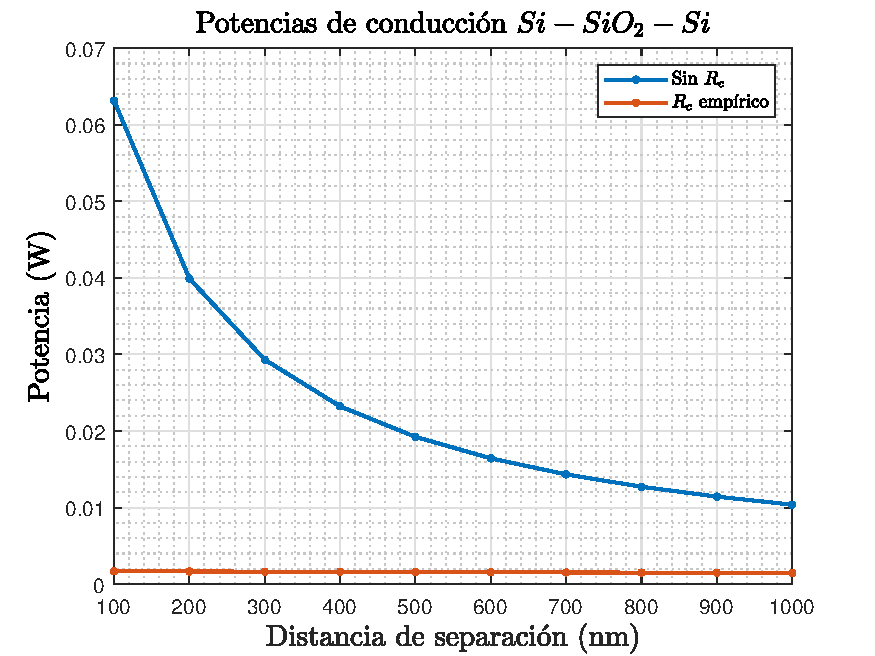
\includegraphics[width=1.0\textwidth]{figuras/Resultados/conduccion/pdf/Prc_SiSiO2Si.pdf}
		\caption{Potencias con y sin $R_c$}
		\label{fig:Prc_SiSiO2Si}
	\end{subfigure}
	\hfill
	\begin{subfigure}[b]{0.49\textwidth}
		\centering
		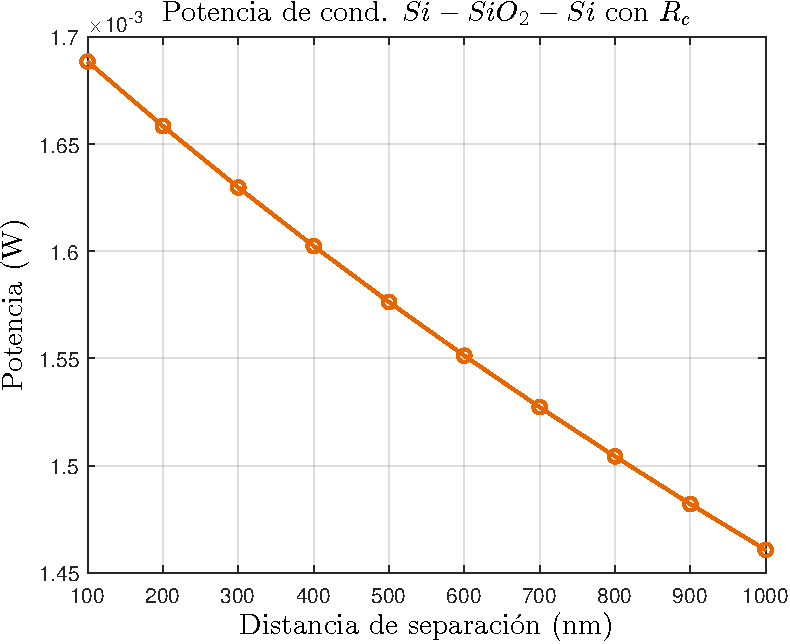
\includegraphics[width=1.0\textwidth]{figuras/Resultados/conduccion/pdf/Prc2_SiSiO2Si.pdf}
		\caption{Potencia solo con $R_c$}
		\label{fig:Prc2_SiSiO2Si}
	\end{subfigure}
	\caption[Efectos de la resistencia de contacto sobre el flujo de calor por conducción]{Representación gráfica del flujo de calor por conducción frente a las diferentes alturas del nano-espaciador con y sin $R_c$. (\subref{fig:Prc_SiSiO2Si}) Comparación de la potencia conducida de un nano-espaciador sin $R_c$ y con $R_c$ sobre un mismo eje.(\subref{fig:Prc2_SiSiO2Si})  Potencia conducida de un nano-espaciador con $R_c$.}
	\label{fig:PcondRc_SiSiO2Si}
\end{figure}
Para un área de 9$\mu m^2$ la resistencia de contacto total es aproximadamente de $444.44\cdot 10^3 \ K/W$ comparada con los $85.43\cdot 10^3 \ K/W$ de la mayor resistencia que presenta el nano-espaciador con 1000nm de altura a 25\textdegree C es al menos 5 veces más grande, por lo cual, como se observa en la figura \ref{fig:Prc_SiSiO2Si} la resistencia de contacto constante domina sobre la resistencia del nano-espaciador dando así la forma aproximada de una recta (figura \ref{fig:Prc2_SiSiO2Si}) porque la mayor caída de temperatura se dá en la superficie de contacto, evitando que aumente la temperatura del nano-espaciador variando menos su resistencia térmica (figuras \ref{fig:Pcond_SiSiO2Si_CFD} y \ref{fig:Pcond_SiSiO2Si_Rc_CFD}).
\graphicspath{ {./figuras/Resultados/conduccion/} }
\begin{figure}[H]
	\centering 		% cond sin Rc
	\begin{subfigure}[b]{0.49\textwidth}
	\centering
		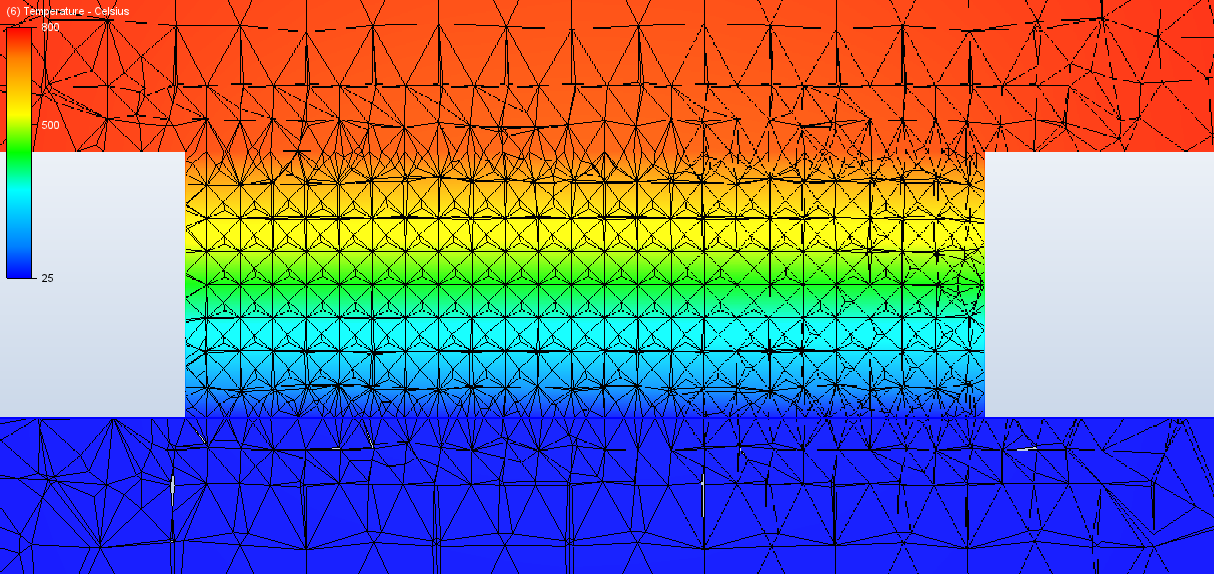
\includegraphics[width=1.00\textwidth]{SiSiO2Si_1000nm_Plane2.png}
		\caption{sin $R_c$}
	\label{fig:Pcond_SiSiO2Si_CFD}
\end{subfigure}
\hfill 					% cond con Rc
\begin{subfigure}[b]{0.49\textwidth}
	\centering
		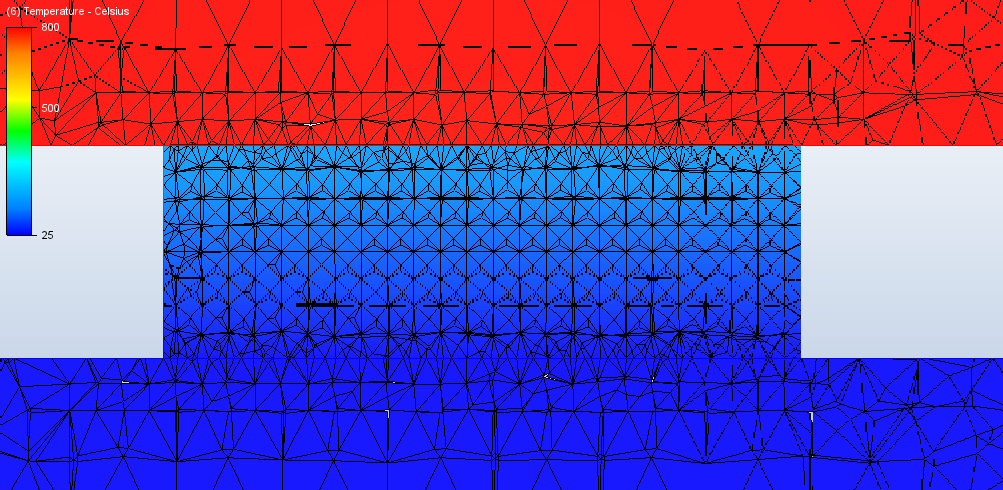
\includegraphics[width=1.00\textwidth]{SiSiO2Si_1000nm_Plane_Rc.png}
		\caption{con $R_c$}
	\label{fig:Pcond_SiSiO2Si_Rc_CFD}
\end{subfigure}
\caption{Resultados gráficos de la simulación de CFD de la transmisión de calor por conducción a través de un nano-espaciador de 1000nm de altura sin $R_c$ (\subref{fig:Pcond_SiSiO2Si_CFD}) y con $R_c$ (\subref{fig:Pcond_SiSiO2Si_Rc_CFD}).}
	\label{fig:Pconds_SiSiO2Si_CFD}
\end{figure}
La disminución de flujo de calor por conducción es significativa para todos los casos, siendo la potencia de conducción con $R_c$ variando aproximadamente entre un 3\% y un 14\% de la potencia sin $R_c$, lo que implica una disminución de conducción de unos 97\% y 85\%.\\\\
Hay que tomar en cuenta que la resistencia de contacto en la realidad no es constante con la temperatura a diferencia de las simulaciones en CFD donde la $R_c$ es constante, pero sirve para tener una primera idea de su importancia en la eliminación de la transferencia de calor por conducción.
\subsection{Efecto de la porosidad sobre la conducción}
\begin{figure}[H]
\centering
	\begin{subfigure}[b]{0.49\textwidth}
		\centering
		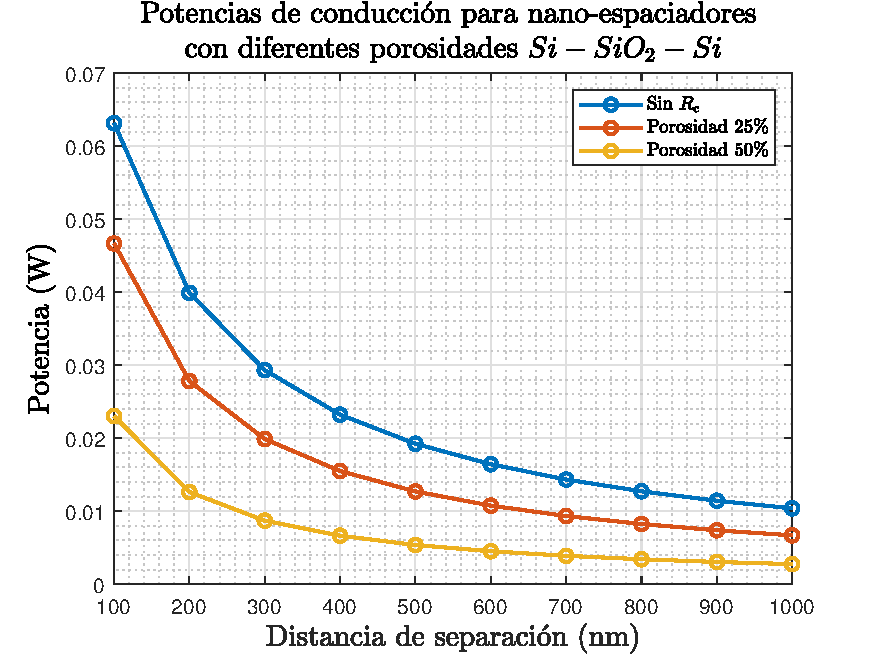
\includegraphics[width=1.0\textwidth]{figuras/Resultados/conduccion/pdf/Ppor_SiSiO2Si.pdf}
		\caption{Efecto de la Porosidad}
		\label{fig:Ppor_SiSiO2Si}
	\end{subfigure}
	\hfill
	\begin{subfigure}[b]{0.49\textwidth}
		\centering
		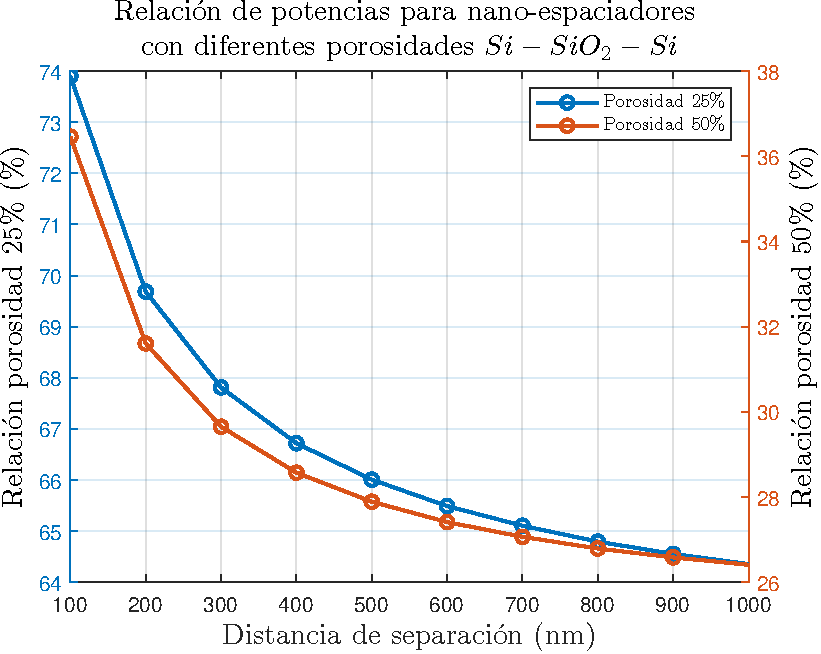
\includegraphics[width=1.0\textwidth]{figuras/Resultados/conduccion/pdf/relPpor_SiSiO2Si.pdf}
		\caption{Efecto de la Porosidad relativo}
		\label{fig:relPpor_SiSiO2Si}
	\end{subfigure}
	\caption[Efectos de la porosidad del nano-espaciador sobre el flujo de calor por conducción]{(\subref{fig:Ppor_SiSiO2Si}) Representación gráfica de las potencias de calor transmitidas por conducción  a través de un nano-espaciador frente a la variación de la altura del nano-espaciador para diferentes grados de porosidad del 0\%, 25\% y 50\% del $SiO_2$ y su modelo analítico (ec. \eqref{eq:Pcond_d_p}). (\subref{fig:relPpor_SiSiO2Si}) Representación gráfica de las relaciones de las potencias por conducción para porosidades del $SiO_2$ de 25\% y 50\% respecto a la potencia de 0\% de porosidad frente a la variación de la altura del nano-espaciador.}
	\label{fig:PcondPor_SiSiO2Si}
\end{figure}
%% Ahora a comentar sobre las porosidades
Para diferentes porosidades la conductividad térmica varía, disminuyendo con el aumento del grado de porosidad \cite{ThermalConductivity_SiO2_2018}, por este motivo la potencia de conducción disminuye para todas las alturas de nano-espaciador. La relación o conductividad térmica normalizada para una porosidad del 25\% y 50\% son respectivamente 0.64 y 0.25 veces la conductividad térmica del material \cite{ThermalConductivity_SiO2_2018}.\\\\
Como se puede observar en la figura \ref{fig:Prc2_SiSiO2Si} las relaciones de potencia no se cumplen completamente porque la temperatura en todo el nano-espaciador no es la misma lo que produce que la conductividad térmica a lo largo del espaciador sea distinta. Por tal motivo, al disminuir la altura del nano-espaciador aumenta la relación porque aumenta el gradiente de temperatura.\\\\
Utilizando la aplicación \textbf{Curve Fitting} de MATLAB se obtiene un modelo matemático que relaciona la potencia de conducción respecto a la altura del nano-espaciador ($d$) y la porosidad del material del nano-espaciador ($\rho$), como se muestra en la ecuación \eqref{eq:Pcond_d_p} donde $d$ es en nanómetros.
\begin{equation}
P(d,\rho)=- \frac{  16.47\cdot \rho-11.03 }{d-106.80\cdot \rho +74.68}
\label{eq:Pcond_d_p}
\end{equation}
%% RAD Si-SiO2-Si
\subsection{Radiación de campo cercano}
Para la radiación por campo cercano se utiliza la aplicación descrita en la sección \ref{sec:calc_campo_cercano} para dos placas gruesas de $Si$ para varias separaciones entre ellas. La potencia radiativa (figura \ref{fig:rad_SiSi_ds}) aumenta con la disminución de la distancia de separación como lo indica el componente exponencial en la ecuación \eqref{eq:flujoEvasNF} de \cite{nfTPV_equations}.
\begin{figure}[H]
	\centering
		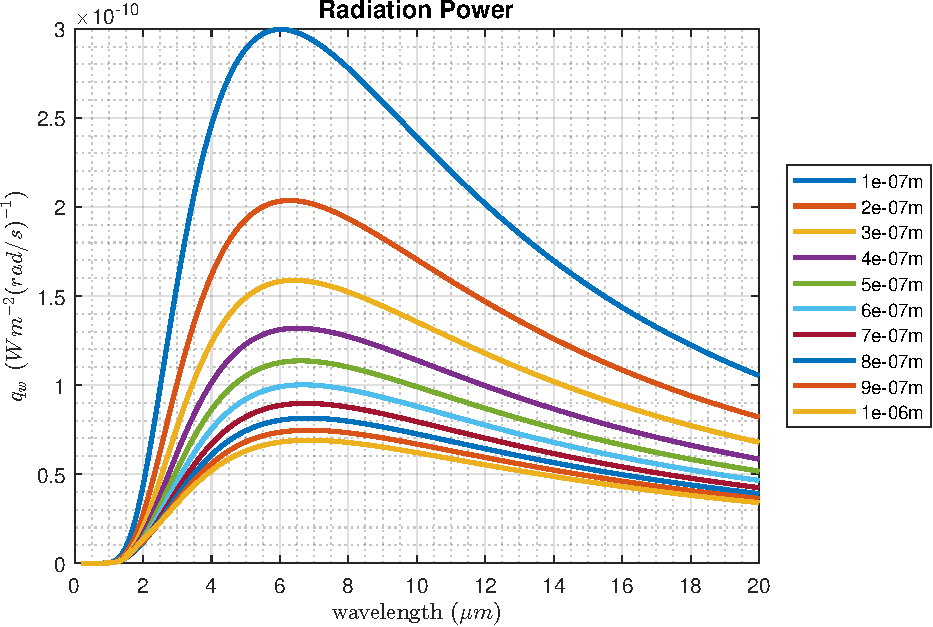
\includegraphics[width=0.7\textwidth]{figuras/Resultados/radiacion/SiSi_ds.pdf}
	\caption{Potencia de radiación monocromática para dos placas gruesas planas de $Si$ en todo el rango espectral frente a diferentes distancias de separación de las placas ($d$) en metros.}
	\label{fig:rad_SiSi_ds}
\end{figure}
Integrando la potencia en el rango espectral de longitudes de onda con energías mayores a 1.1 eV, energía de banda del $Si$, se obtiene en promedio potencias del orden de $60 \ W/m^2$ (figura \ref{fig:prad_Eg11_SiSi}) a diferencia de integrar en todo el rango espectral, hasta las $\sim$20 $\mu m$, cuyo orden es de $10^4 \ W/m^2$ (figura \ref{fig:prad_full_SiSi}), Lo cual indica que se desaprovecha una gran cantidad de energía.
\begin{figure}[H]
	\centering
		\begin{subfigure}[b]{0.49\textwidth}
	\centering
		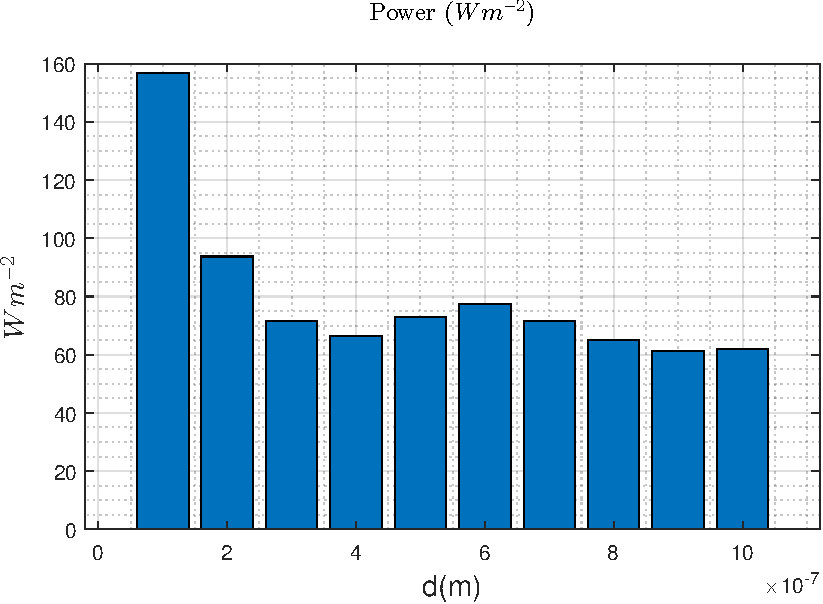
\includegraphics[width=1.00\textwidth]{figuras/Resultados/radiacion/p_11_SiSi.pdf}
	\caption{Potencia para energía mayor a 1.1 eV}
	\label{fig:prad_Eg11_SiSi}
\end{subfigure}
\hfill
\begin{subfigure}[b]{0.49\textwidth}
	\centering
		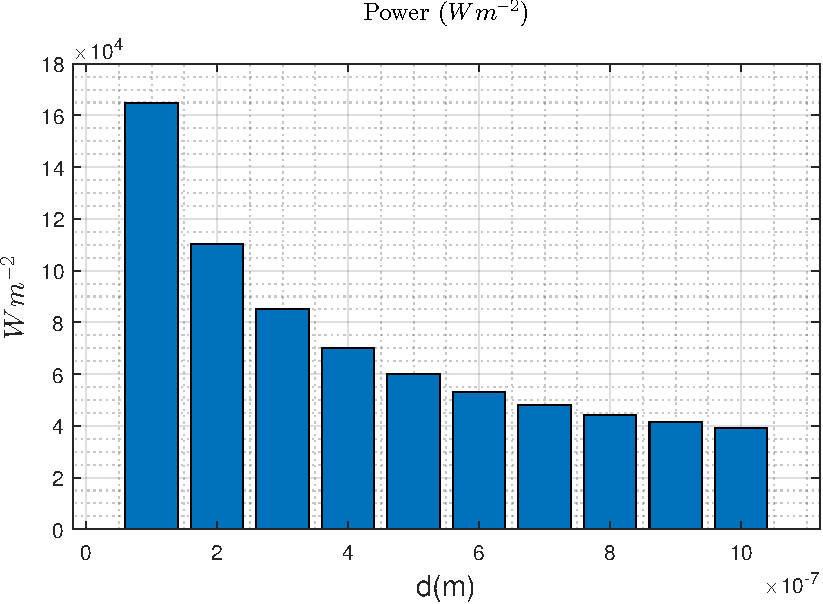
\includegraphics[width=1.00\textwidth]{figuras/Resultados/radiacion/p_full_SiSi.pdf}
	\caption{Potencia hasta las $\sim$20 $\mu m$}
	\label{fig:prad_full_SiSi}
\end{subfigure}
	\caption{Potencias por unidad de área transmitida por radiación por efecto de campo cercano para el rango espectral de energía mayor a 1.1 eV (\subref{fig:prad_Eg11_SiSi}) y para todo el rango espectral (\subref{fig:prad_full_SiSi}) frente a las diferentes distancias de separación.}
	\label{fig:prad_SiSi}
\end{figure}
Las potencias radiadas obtenidas para el rango de longitudes de onda mayor a la bandgap del $Si$ son muy pequeñas (figura \ref{fig:prad_Eg11_SiSi}), produciendo que no sea viable este sistema porque las pérdidas por conducción son demasiado grandes. Esto se puede visualizar en la figura \ref{fig:rel_SiSi11_Rc}, donde ni siquiera asumiendo la presencia de un único nano-espaciador con Rc se consigue que la potencia radiada sea al menos un orden de magnitud más alta que la potencia transferida por conducción (no se alcanza un factor 10).
\begin{figure}[H]
	\centering
\begin{subfigure}[b]{0.49\textwidth}
	\centering
		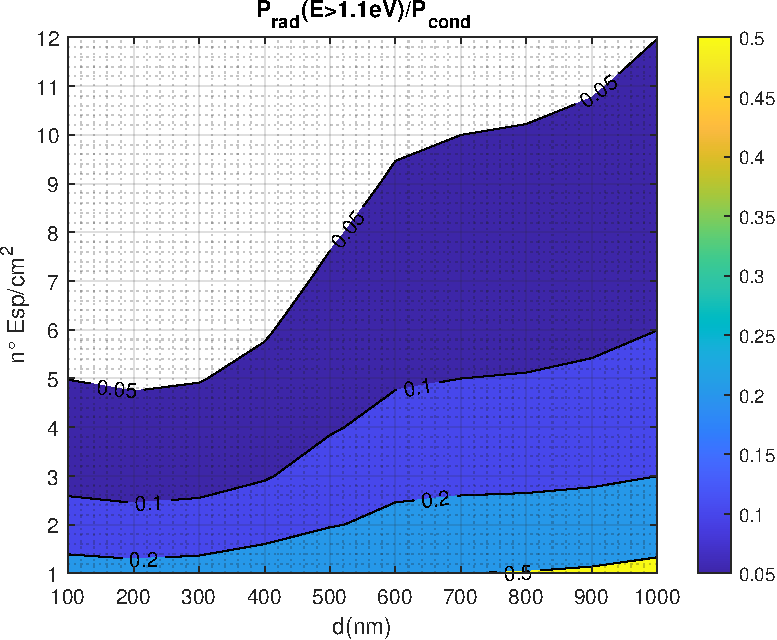
\includegraphics[width=1.00\textwidth]{figuras/Resultados/RelacionCondRad/rel_SiSi11.pdf}
	\caption{Relación de potencias para Eg$>$1.1 eV}
	\label{fig:rel_SiSi11}
\end{subfigure}
\hfill
\begin{subfigure}[b]{0.49\textwidth}
	\centering
		\includegraphics[width=1.00\textwidth]{figuras/Resultados/RelacionCondRad/rel_SiSi11_Rc.pdf}
	\caption{Relación de potencias para Eg$>$1.1 eV con $R_c$}
	\label{fig:rel_SiSi11_Rc}
\end{subfigure}
\caption{Densidad de los nano-espaciadores para diferentes relaciones de las potencias de radiación en el rango espectral de energía mayor a 1.1 eV respecto a las de conducción para cada densidad de nano-espaciadores de un sistema nTPV de 1$cm^2$ y célula de $Si$ sin $R_c$ (\subref{fig:rel_SiSi11}) y con $R_c$ (\subref{fig:rel_SiSi11_Rc}) frente a las diferentes alturas de los nano-espaciadores. La barra de colores al lateral de cada gráfica representa todas las relaciones entre ambas potencias para diferentes densidades de nano-espaciadores en el rango que se muestra en los extremos de cada barra. También se muestran los contornos con su valor para destacar las distintas relaciones existentes de una manera sencilla.}
	\label{fig:rels_SiSi11}
\end{figure}
%% RELACION ENTRE COND Y RAD
Para tener una primera mejor idea de los valores numéricos de los resultados obtenidos de las simulaciones de transmisión de calor por conducción y radiación de campo cercano se recopilan en la tabla \ref{tab:condTerSiSiO2Si}, estando en notación científica y con los decimales necesarios para una clara diferenciación de los resultados con el cambio de la distancia de separación entre emisor y célula.
\begin{table}[H]
	\centering
		\begin{tabular}{|c||c|c|c|c||c|c|}
		\hline
			\multirow{2}{*}{ }& \multicolumn{6}{c|}{\textbf{\large Potencias según como se transmite el calor}}\\ \cline{2-7}
		  & \multicolumn{4}{c||}{Conducción (W/nº nano-espaciadores)}& \multicolumn{2}{c|}{Radiación $(W/m^2)$}\\ \hline
			Dist. (nm)&$P_{Normal}$&$P_{R_c-Empirico}$&$P_{Porosidad25}$&$P_{Porosidad50}$&$P_{Eg>1.1eV}$&$P_{full}$\\ \hline \hline
			100&6,31E-02&1,69E-03&4,67E-02&2,30E-02&156.89&1,65E+05\\ \hline
			200&3,99E-02&1,66E-03&2,78E-02&1,26E-02&93.75&1,10E+05\\ \hline
			300&2,93E-02&1,63E-03&1,99E-02&8,69E-03&71.75&8,51E+04\\ \hline
			400&2,32E-02&1,60E-03&1,55E-02&6,63E-03&66.39&7,01E+04\\ \hline
			500&1,92E-02&1,58E-03&1,27E-02&5,36E-03&73.00&6,02E+04\\ \hline
			600&1,64E-02&1,55E-03&1,08E-02&4,50E-03&77.52&5,32E+04\\ \hline
			700&1,43E-02&1,53E-03&9,33E-03&3,88E-03&71.63&4,80E+04\\ \hline
			800&1,27E-02&1,50E-03&8,24E-03&3,41E-03&64.90&4,43E+04\\ \hline
			900&1,14E-02&1,48E-03&7,38E-03&3,04E-03&61.42&4,14E+04\\ \hline
		 1000&1,04E-02&1,46E-03&6,68E-03&2,74E-03&62.09&3,93E+04\\ \hline
		\end{tabular}
	\caption{Tabla de resultados de las simulaciones de conducción y radiación de campo cercano para diferentes alturas del nano-espaciador. Flujos de calor del nTPV $Si-SiO_2-Si$ para diferentes alturas del nano-espaciador, para los casos sin $R_c$ y con $R_c$ igual a $4 \cdot 10^{-6} \ m^2 K/W$ \cite{nf_TPV_Pillars_SiO2}, y sin $R_c$ pero con las proporciones de las porosidades de \cite{ThermalConductivity_SiO2_2018} para un 25\% y un 50\%.}
	\label{tab:condTerSiSiO2Si}
\end{table}
\vfill \newpage
%%% AHORA EL CASO DE Si SiO2 y Ge
\section{Resultados de las simulaciones para una nTPV de Si-SiO2-Ge}\label{sec:res_SiSiO2Ge}
A continuación se procede a estudiar un caso más realista del sistema nTPV descrito en la sección anterior con una célula de $Ge$ en vez de una de $Si$, cuya bandgap es de 0.7 eV respecto a los 1.1 eV del $Si$.
\subsection{Simulaciones de CFD}
Se realizan las simulaciones de transmisión de calor por conducción en CFD, obteniéndose una reducción considerable de la potencia de la nTPV con $R_c$ (figura \ref{fig:Prc_SiSiO2Ge}) respecto a sin $R_c$ (figura \ref{fig:Pn_SiSiO2Ge}), como en el caso de la célula de $Si$ (figuras \ref{fig:PcondRc_SiSiO2Si} \subref{fig:Prc_SiSiO2Si} y \subref{fig:Prc2_SiSiO2Si}).
\graphicspath{ {./figuras/Resultados/conduccion/pdf/} }
\begin{figure}[H]
	\centering
	%% Si-SiO2-Si Eg
	\begin{subfigure}[b]{0.49\textwidth}
		\centering
		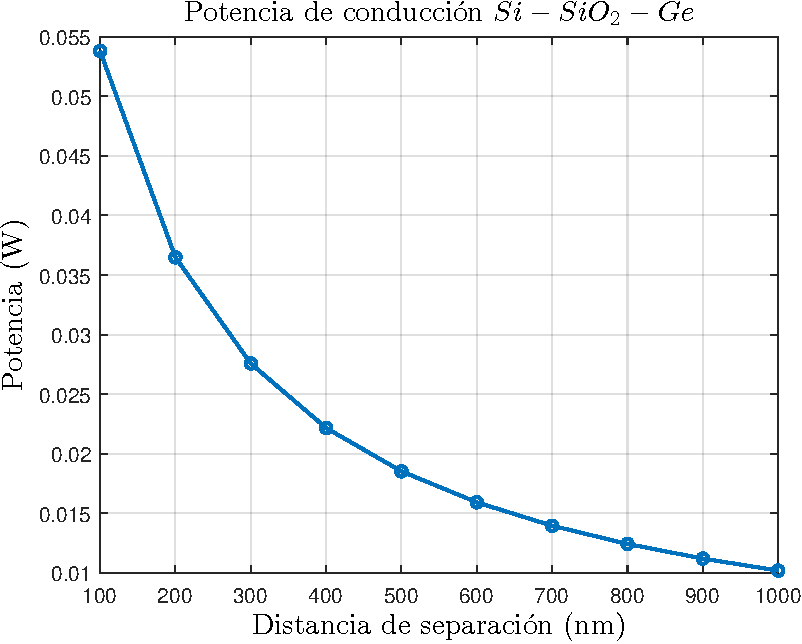
\includegraphics[width=1\textwidth]{Pn_SiSiO2Ge.pdf}
		\caption{Potencia cond. sin $R_c$}
		\label{fig:Pn_SiSiO2Ge}
	\end{subfigure}
	\hfill
	\begin{subfigure}[b]{0.49\textwidth}
		\centering
		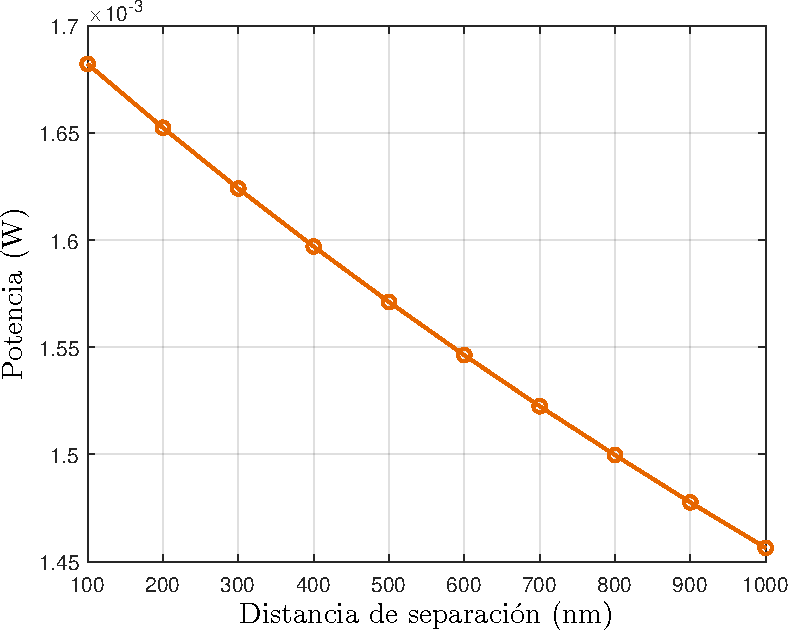
\includegraphics[width=1.00\textwidth]{Prc2_SiSiO2Ge.pdf}
		\caption{Potencia cond. con $R_c$}
		\label{fig:Prc_SiSiO2Ge}
	\end{subfigure}
	\caption{Potencias de conducción para un sistema nTPV de $Si-SiO_2-Ge$ de un nano-espaciador con emisor a 800\textdegree C y célula a 25\textdegree C sin $R_c$ (\subref{fig:Pn_SiSiO2Ge}) y con $R_c$ (\subref{fig:Prc_SiSiO2Ge}) frente a las diferentes alturas del nano-espaciador.}
	\label{fig:Pcond_SiSiO2Ge}
\end{figure}
La potencia de conducción con $R_c$ disminuye de unos 53.80 $mW$ sin $R_c$ a unos 1.68 $mW$ para una altura de nano-espaciador de 100nm, que representa una relación del 3.13\%. Para unos 1000nm de altura de nano-espaciador la potencia disminuye de unos 10.20 $mW$ sin $R_c$ a unos 1.46 $mW$ con $R_c$, que representa una relación del 14.31\%.\\\\
Comparando los resultados obtenidos de la simulación de transmisión de calor por conducción de la nTPV de célula de $Ge$ respecto a la de $Si$, ambas con $R_c$, se obtiene una relación mayor del 99\% para todas las alturas del nano-espaciador, dando a entender que la diferencia de la conductividad térmica de los materiales no produce un efecto significativo sobre la conducción con la existencia de $R_c$, a diferencia de la nTPV sin $R_c$ donde la relación varía entre un $\sim$85\% y un $\sim$98\%.
\vfill
\subsection{Radiación de campo cercano}
De las simulaciones de radiación de campo cercano se obtienen también resultados muy parecidos a los obtenidos en el caso de la célula de $Si$ (figura \ref{fig:SiSi_vs_SiGe}), solo mostrándose hasta los $\sim$14$\mu m$ de longitud de onda, donde se observa como al disminuir la distancia de separación aumenta la potencia radiativa (figura \ref{fig:rad_SiGe}).
\begin{figure}[H]
\centering
\begin{subfigure}[b]{0.49\textwidth}
	\centering
		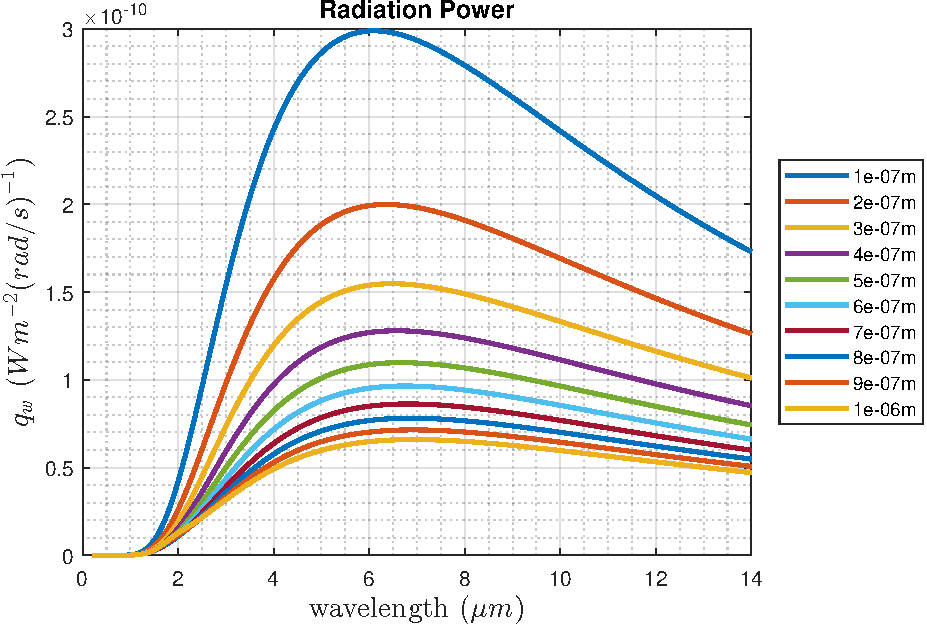
\includegraphics[width=1.00\textwidth]{figuras/Resultados/radiacion/SiGe.pdf}
	\caption{Potencia monocromática para varias $d$}
	\label{fig:rad_SiGe}
\end{subfigure}
\hfill
\begin{subfigure}[b]{0.49\textwidth}
	\centering
		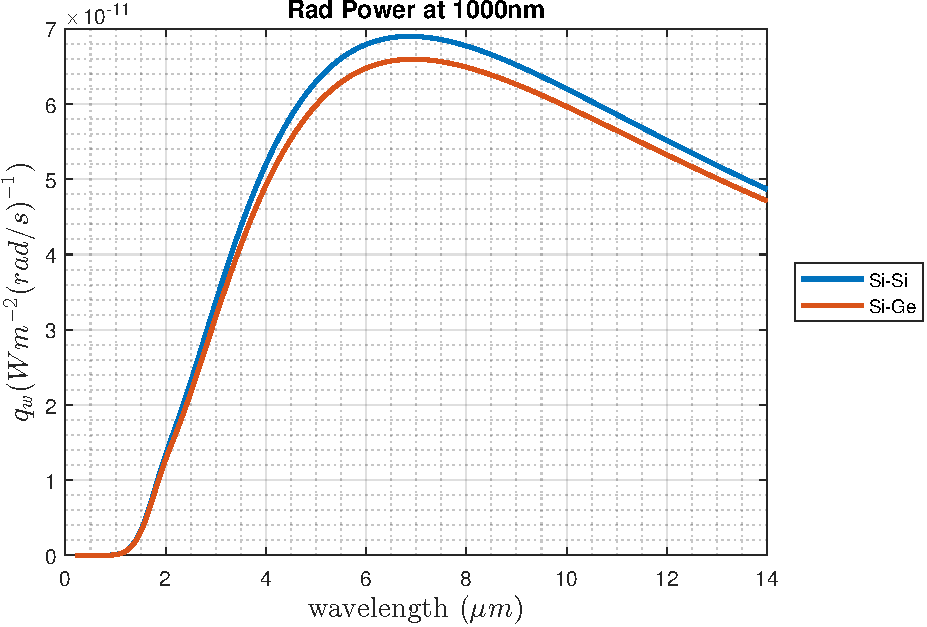
\includegraphics[width=1.00\textwidth]{figuras/Resultados/radiacion/SiSi_vs_SiGe.pdf}
	\caption{Comparación de células de $Si$ y $Ge$}
	\label{fig:SiSi_vs_SiGe}
\end{subfigure}
\caption{Potencias de radiación monocromática por campo cercano para un sistema nTPV $Si-SiO_2-Ge$ frente a las longitudes de onda para varias distancias de separación entre placas(\subref{fig:rad_SiGe}) y para dos materiales de célula, $Si$ y $Ge$ (\subref{fig:SiSi_vs_SiGe}).}
\label{fig:rads_SiGe}
\end{figure}
Para la obtención de las potencias de radiación se procede a realizar la integral en el rango espectral de energía mayor a los 0.7 eV, obteniéndose potencias alrededor de los $10^3 \ W/m^2$ (figura \ref{fig:p_Eg_SiGe}), y para todo el rango espectral de longitudes de onda se obtiene potencias alrededor de los $10^4 \ W/m^2$ con un máximo de $\sim$1.5$10^5 \ W/m^2$ (figura \ref{fig:p_full_SiGe} y tabla \ref{tab:SiSiO2Ge}). 
%% POTENCIAS INTEGRADAS
\begin{figure}[H]
\centering
\begin{subfigure}[b]{0.49\textwidth}
	\centering
		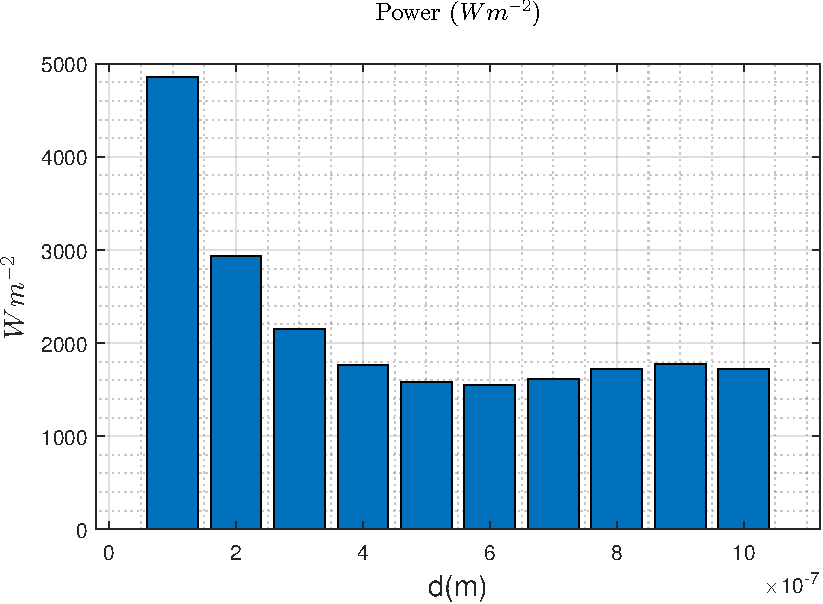
\includegraphics[width=1.00\textwidth]{figuras/Resultados/radiacion/p_Eg_SiGe.pdf}
	\caption{Potencia para Eg$>$0.7eV}
	\label{fig:p_Eg_SiGe}
\end{subfigure}
\hfill
\begin{subfigure}[b]{0.49\textwidth}
	\centering
		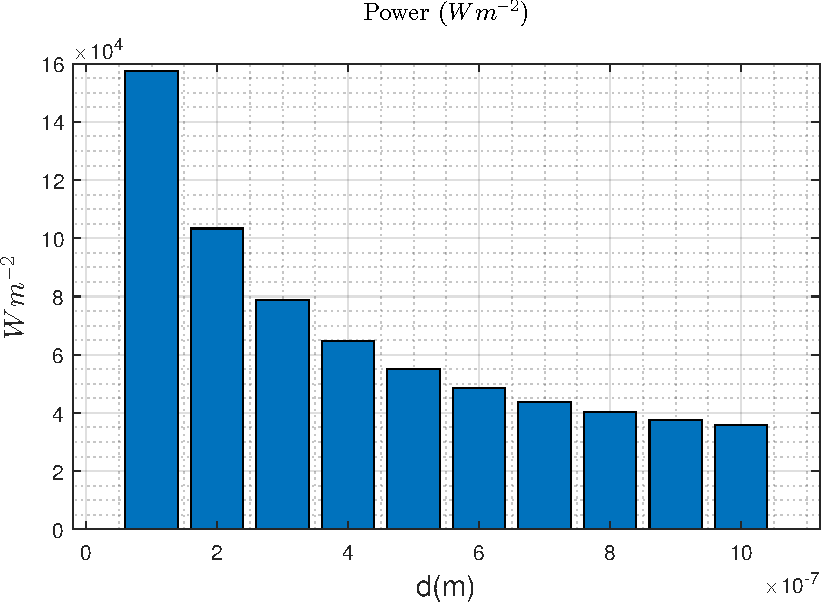
\includegraphics[width=1.00\textwidth]{figuras/Resultados/radiacion/p_full_SiGe.pdf}
	\caption{Potencia hasta $\sim$14$\mu m$}
	\label{fig:p_full_SiGe}
\end{subfigure}
	\caption[Potencias por unidad de área para la radiación de campo cercano para el sistema $Si-SiO_2-Ge$ frente a las diferentes alturas del nano-espaciador]{Potencias por unidad de área para la radiación de campo cercano para el sistema $Si-SiO_2-Ge$ frente a las diferentes alturas del nano-espaciador. (\subref{fig:p_Eg_SiGe}) Potencias en el rango espectral de todas las longitudes de onda de energía mayor a 0.7 eV. (\subref{fig:p_full_SiGe}) Potencias en todo el rango espectral, hasta las $\sim$14$\mu m$.}
	\label{fig:p_SiGe}
\end{figure}
Como para el caso de la nTPV de $Si-SiO_2-Si$ la diferencia de la potencia entre integrar hasta los 0.7 eV del rango espectral e integrar en todo el rango espectral es significativa. Al cambiar la célula de $Si$ por una de menor bandgap de $Ge$ se aumenta la cantidad de potencia que se puede convertir en electricidad. También se observa una disminución de las potencias alrededor de los 600nm (figura \ref{fig:p_Eg_SiGe}), a diferencia de la célula de $Si$ que aumenta (\ref{fig:prad_Eg11_SiSi}).
%%%   DENSIDAD DE NANO-ESPACIADORES
\subsection{Densidad de nano-espaciadores}
Para tener una mejor percepción de las ventajas que presenta el usar una célula de $Ge$ frente a una de $Si$ se calcula la densidad de nano-espaciadores frente a las alturas del nano-espaciador para todas las relaciones de la potencia de radiación respecto a la de conducción mayores que 3 o 10.\\\\
Hay que tener en cuenta que para un centímetro cuadrado de superficie de radiación la transmisión de calor por radiación se ve multiplicado por $10^{-4}$, por lo tanto, la potencia de radiación con $E_g>0.7eV$ en un centímetro cuadrado es $\sim$10 mayor que la potencia conducida sin resistencia de contacto para un nano-espaciador (figura \ref{fig:rel_SiSiO2Ge}), pero $\sim$100 veces mayor que la potencia conducida con resistencia de contacto (figura \ref{fig:rel_SiSiO2Ge_Rc}).
\begin{figure}[H]
	\centering
	%% Si-SiO2-Si Eg
	\begin{subfigure}[b]{0.49\textwidth}
		\centering
		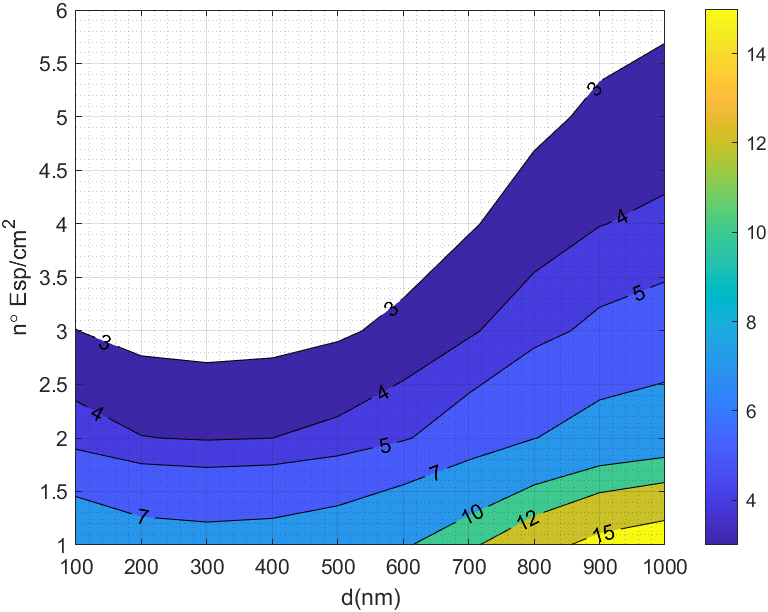
\includegraphics[width=1.00\textwidth]{figuras/Resultados/RelacionCondRad/SiGe.png}
		\caption{$E>0.7eV$, sin $R_c$}
		\label{fig:rel_SiSiO2Ge}
	\end{subfigure}
	\hfill
	\begin{subfigure}[b]{0.49\textwidth}
			\centering
			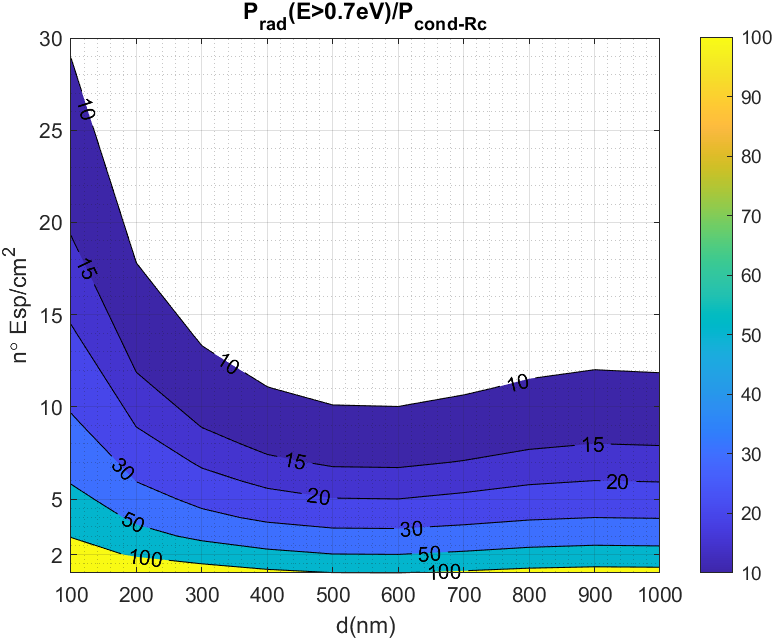
\includegraphics[width=1.00\textwidth]{figuras/Resultados/RelacionCondRad/SiGe_Rc.png}
			\caption{$E>0.7eV$, con $R_c$}
			\label{fig:rel_SiSiO2Ge_Rc}
		\end{subfigure}
	\caption{Densidad de nano-espaciadores por $cm^2$ frente a las alturas de los nano-espaciadores para todas las relaciones de la potencia de radiación en el rango espectral de energías mayores e igual a 0.7 eV respecto a las potencias de conducción (dependencia en la densidad de nano-espaciadores) mayores a 3 para el caso sin $R_c$ (\subref{fig:rel_SiSiO2Ge}) y mayores a 10 para el caso con $R_c$ (\subref{fig:rel_SiSiO2Ge_Rc}). Donde las barras de colores laterales representan los colores asociados a cada uno de los valores de las relaciones de las potencias, con los contornos de las relaciones más significativas en los gráficos.}
	\label{fig:relation_SiSiO2Ge}
\end{figure}
Como se observa en las figuras \ref{fig:relation_SiSiO2Ge} \subref{fig:rel_SiSiO2Ge} y \subref{fig:rel_SiSiO2Ge_Rc}, la forma de la curva cambia su tendencia según se incluya o no la $R_c$ porque sin $R_c$ la tendencia de la curva de crecer con el aumento de la altura de los nano-espaciadores está marcada por la potencia de conducción (inversamente proporcional), y para el caso con $R_c$ la  tendencia de la curva de aumentar con la disminución de la altura de los nano-espaciadores está marcada por la potencia de radiación de campo cercano.\\\\
Los valores de las relaciones entre ambas potencias no son muy altos para el caso sin $R_c$, apenás consiguiendo seguro un factor de relación de al menos un orden de magnitud solo para una altura de un nano-espaciador de al menos unos 600nm, a diferencia del caso con $R_c$ que se consigue como mínimo una relación de dos ordenes de magnitud para todas las alturas de un nano-espaciador. Estas relaciones disminuyen con el aumento de la densidad de los nano-espaciadores porque aumenta la potencia de conducción, por este motivo solo serán viables aquellas configuraciones que como mínimo tengan una relación de potencias de un orden de magnitud para una configuración mínima de cuatro nano-espaciadores.\\\\
Para la densidad de nano-espaciadores se nota en la figura \ref{fig:rel_SiSiO2Ge_Rc} que el valor máximo para una relación de potencias de un orden de magnitud es aproximadamente 30, que es aproximadamente 10 veces respecto a la del caso sin $R_c$ (menor que 3) para la misma altura de nano-espaciadores (figura \ref{fig:rel_SiSiO2Ge}), y el valor para la misma relación de potencias para una altura de nano-espaciadores de 1000nm es 12, que es entre 6 y 12 veces respecto al caso sin $R_c$.\\\\
Por lo tanto, entre ambos casos el que puede ser viable es el sistema nTPV con $R_c$ porque presenta una mayor densidad de nano-espaciadores para una misma relación de potencias, lo que permite que se distribuya la carga sobre los nano-espaciadores y sea más fácil mantener la separación entre el emisor y la célula constante sobre toda la superficie.
\begin{figure}[H]
		\begin{subfigure}[b]{0.49\textwidth}
		\centering
		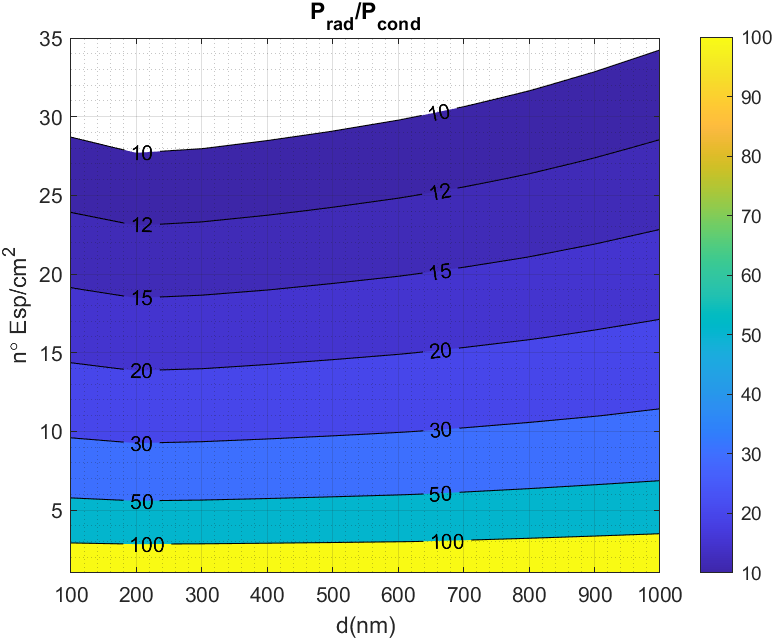
\includegraphics[width=1.00\textwidth]{figuras/Resultados/RelacionCondRad/SiGe_full.png}
		\caption{rango completo, sin $R_c$}
		\label{fig:rel_SiSiO2Ge_full}
	\end{subfigure}
		\hfill
		\begin{subfigure}[b]{0.49\textwidth}
			\centering
			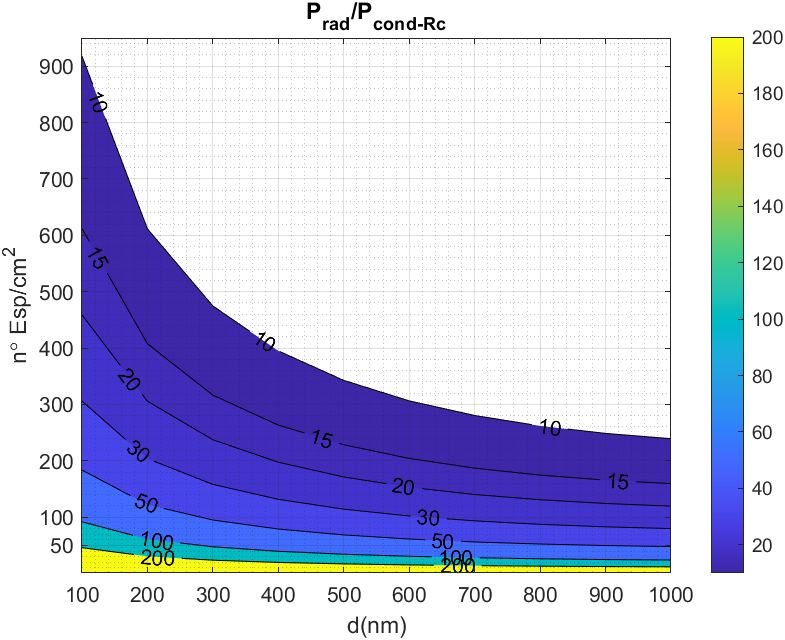
\includegraphics[width=1.00\textwidth]{figuras/Resultados/RelacionCondRad/SiGe_Rc_full_10.png}
			\caption{rango completo, con $R_c$}
			\label{fig:rel_SiSiO2Ge_Rc_full}
		\end{subfigure}
	\caption{Densidad de nano-espaciadores por $cm^2$ frente a las alturas de los nano-espaciadores para todas las relaciones de la potencia de radiación en todo el rango espectral respecto a las potencias de conducción (dependencia en la densidad de nano-espaciadores) mayores a 10 para el caso sin $R_c$ (\subref{fig:rel_SiSiO2Ge_full}) y para el caso con $R_c$ (\subref{fig:rel_SiSiO2Ge_Rc_full}). Donde las barras de colores laterales representan los colores asociados a cada uno de los valores de las relaciones de las potencias, con los contornos de las relaciones más significativas en los gráficos.}%
	\label{fig:rels_SiSiO2Ge_full}%
\end{figure}
Por último, se representan el caso de la densidad de nano-espaciadores frente a las alturas de los nano-espaciadores para varias relaciones de las potencias de radiación en todo el rango espectral y las potencias de conducción sin y con $R_c$ (figuras \ref{fig:rels_SiSiO2Ge_full}  \subref{fig:rel_SiSiO2Ge_full} y \subref{fig:rel_SiSiO2Ge_Rc_full}, respectivamente), observándose las mismas tendencias que para el rango espectral de energías mayores e iguales a 0.7 eV pero con mayor densidad de nano-espaciadores por el aumento de la potencia radiada de campo cercano, por lo tanto, el aumento del rango espectral de radiación útil es bastante importante para el aumento de la potencia a convertir en electricidad.\\\\
Para facilitar la revisión de los resultados obtenidos de las simulaciones y de los cálculos realizados se recopilan en la tabla \ref{tab:SiSiO2Ge}, donde se presentan en notación científica para facilitar la observación de los ordenes de magnitud de los resultados.
\begin{table}[H]
	\centering
		\begin{tabular}{|c||c|c||c|c|}
		\hline
\multirow{2}{*}{ }& \multicolumn{4}{c|}{\textbf{\large Potencias según transmisión del calor}}\\ \cline{2-5}
& \multicolumn{2}{c||}{Conducción (W/nº esp.)}& \multicolumn{2}{c|}{Radiación $(W/m^2)$}\\ \hline
Dist. (nm)&$P_{Normal}$&$P_{R_c-Empirico}$&$P_{Eg>0.7eV}$&$P_{full}$\\ \hline \hline
100&5,38E-02&1,68E-03&4,87E+03&1,54E+05\\ \hline 
200&3,65E-02&1,65E-03&2,94E+03&1,01E+05\\ \hline 
300&2,76E-02&1,62E-03&2,16E+03&7,71E+04\\ \hline 
400&2,22E-02&1,60E-03&1,77E+03&6,31E+04\\ \hline 
500&1,85E-02&1,57E-03&1,59E+03&5,38E+04\\ \hline 
600&1,59E-02&1,55E-03&1,55E+03&4,74E+04\\ \hline 
700&1,39E-02&1,52E-03&1,62E+03&4,27E+04\\ \hline 
800&1,24E-02&1,50E-03&1,73E+03&3,93E+04\\ \hline 
900&1,12E-02&1,48E-03&1,78E+03&3,67E+04\\ \hline 
1000&1,02E-02&1,46E-03&1,73E+03&3,49E+04\\ \hline 
		\end{tabular}
	\caption{Tabla de las potencias de resultado de las simulaciones de transmisión de calor por radiación de campo cercano y conducción para el sistema nTPV $Si-SiO_2-Ge$.}
	\label{tab:SiSiO2Ge}
\end{table}
\vfill
%%% RESULTADOS DE SS
\newpage
\section{Resultados de las simulaciones para una nTPV de SS-SiO2-Ge}\label{sec:res_SsSiO2Ge}
Una de las razones más importantes del estudio de las nTPV es la recuperación de calor residual, por lo cual se simula la transmisión por conducción y radiación para una nTPV de emisor de acero inoxidable ($SS$) porque es un material altamente utilizado en todos los sectores, principalmente en la industria, ya sea en calderas, tuberías u otros componentes o máquinas se encuentran a altas temperaturas.
\subsection{Simulaciones de CFD}
Para las simulaciones de transmisión de calor por conducción se estudian los efectos de resistencias de contacto aún mayores a la empírica estudiada hasta ahora. Las nuevas resistencias de contacto se obtienen aplicando la inversa a la conductancia de contacto ($h_c=1/R_c$), la cual se obtiene mediante la relación de las conductancias de contacto según la ecuación \eqref{eq:relacion_conductividadesTermicas} para un emisor de $SS$ y un nano-espaciador liso de $SiO_2$. La conductancia de contacto entre dos aceros inoxidables utilizada para una presión de $\sim$1 GPa, porque a dicha presión el error respecto al modelo matemático es pequeño, es aproximadamente unos 1000 $W/(m^2 K)$ \cite{experimental_Rc_SS}.\\\\
La nueva resistencia de contacto calculada a partir de la conductancia de contacto entre dos aceros inoxidables es $5.5\cdot 10^{-3} \ m^2 K/W$ y se toma un valor intermedio entre dicha resistencia de contacto y la resistencia de contacto empírica de $4\cdot 10^{-6} \ m^2 K/W$ \cite{nf_TPV_Pillars_SiO2} para obtener en mayor detalle los efectos de la resistencia de contacto sobre el flujo de calor por conducción, siendo el valor de dicha resistencia de contacto calculada intermedia unos $\sim 2.75\cdot 10^{-3} \ m^2 K/W$.
\graphicspath{ {./figuras/Resultados/conduccion/pdf/} }
\begin{figure}[H]
	\centering
	\begin{subfigure}[b]{0.49\textwidth}
		\centering
			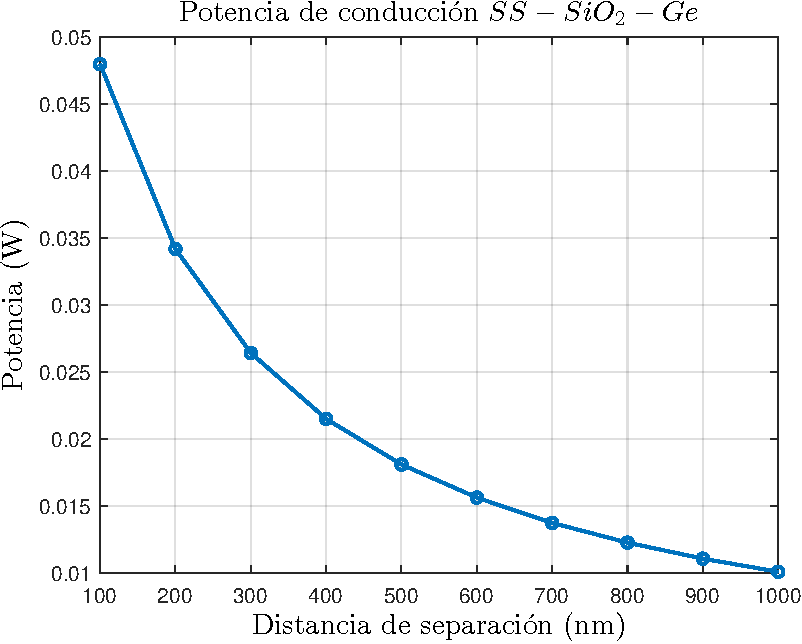
\includegraphics[width=1.00\textwidth]{Pn_SsSiO2Ge.pdf}
		\caption{ }
		\label{fig:Pn_SsSiO2Ge}
	\end{subfigure}
	\hfill
	\begin{subfigure}[b]{0.49\textwidth}
		\centering
			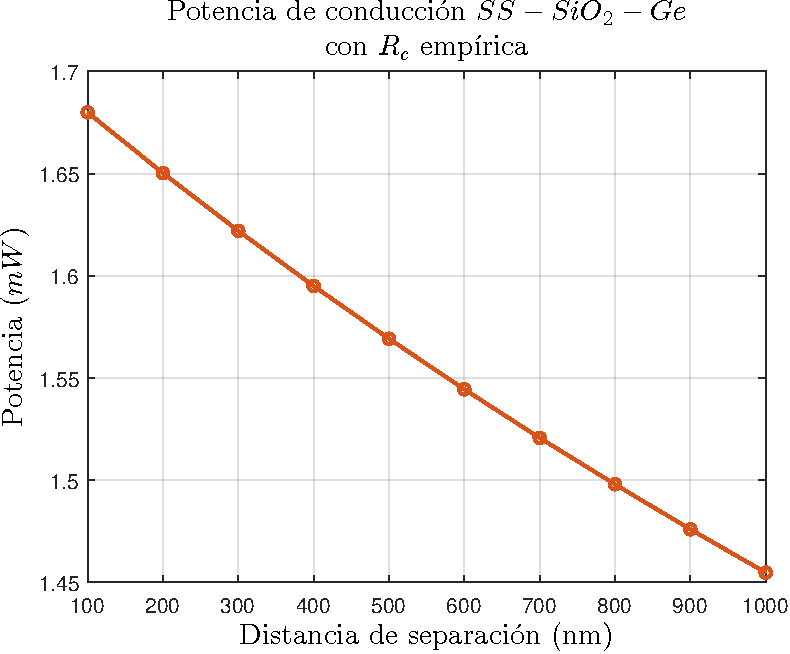
\includegraphics[width=1.00\textwidth]{Prc_SsSiO2Ge_Emp.pdf}
		\caption{ }
		\label{fig:Prc_SsSiO2Ge_Emp}
	\end{subfigure}
	\caption{Potencias por conducción para una nTPV $SS-SiO_2-Ge$ sin $R_c$ (\subref{fig:Pn_SsSiO2Ge}) y con $R_c$ empírica de $4\cdot 10^{-6} \ m^2 K/W$ (\subref{fig:Prc_SsSiO2Ge_Emp}) frente a las alturas de un nano-espaciador.}
	\label{fig:Pcond1_SsSiO2Ge}
\end{figure}
La potencia máxima sin $R_c$ es menor que 0.05W (figura \ref{fig:Pn_SsSiO2Ge}) a diferencia de la nTPV de $Si-SiO_2-Ge$ que la potencia máxima es menor a unos 0.055W (figura \ref{fig:Pn_SiSiO2Ge}). Para la nTPV con $R_c$ empírica la potencia conducida se encuentra en el rango de 1.45 $mW$ a 1.7 $mW$ (figura \ref{fig:Prc_SsSiO2Ge_Emp}), igual que para el caso de la nTPV de $Si-SiO_2-Ge$, por lo tanto, el material del emisor no es significativo cuando existe una resistencia de contacto de por lo menos $4\cdot 10^{-6} \ m^2 K/W$.\\\\
Para las resistencias de contacto calculadas la potencia por conducción disminuye significativamente, siendo tres ordenes de magnitud menor que para la $R_c$ empírica, correspondiente a los tres ordenes de magnitud por encima que las resistencias de contacto calculadas son respecto a la empírica (figuras \ref{fig:Prc_SsSiO2Ge_Emp} y \ref{fig:Prc_SsSiO2Ge_Inter}). Por ende, la resistencia de contacto es la resistencia de mayor relevancia del sistema nTPV.
\begin{figure}[H]
	\centering
	\begin{subfigure}[b]{0.49\textwidth}
		\centering
			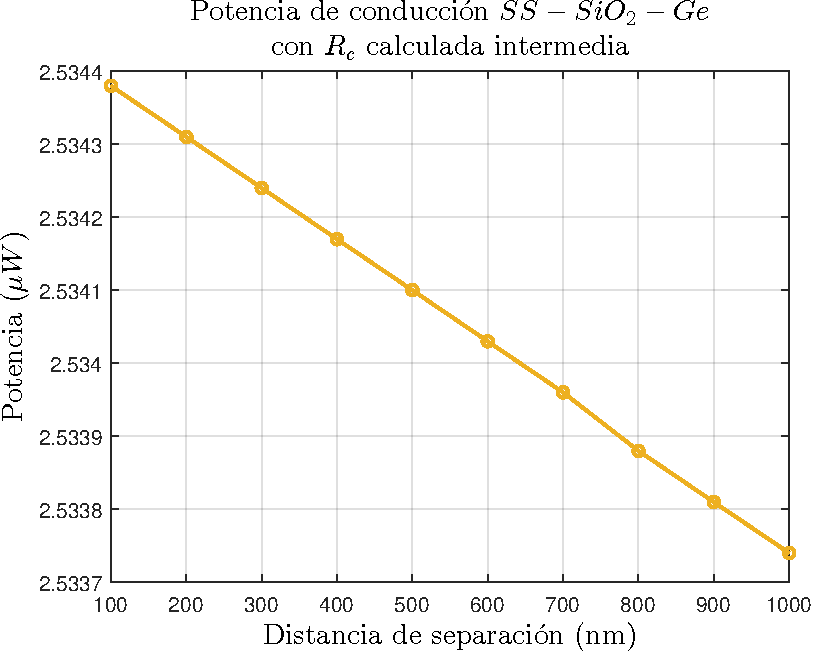
\includegraphics[width=1.00\textwidth]{Prc_SsSiO2Ge_Inter.pdf}
		\caption{ }
		\label{fig:Prc_SsSiO2Ge_Inter}
	\end{subfigure}
	\hfill
	\begin{subfigure}[b]{0.49\textwidth}
		\centering
			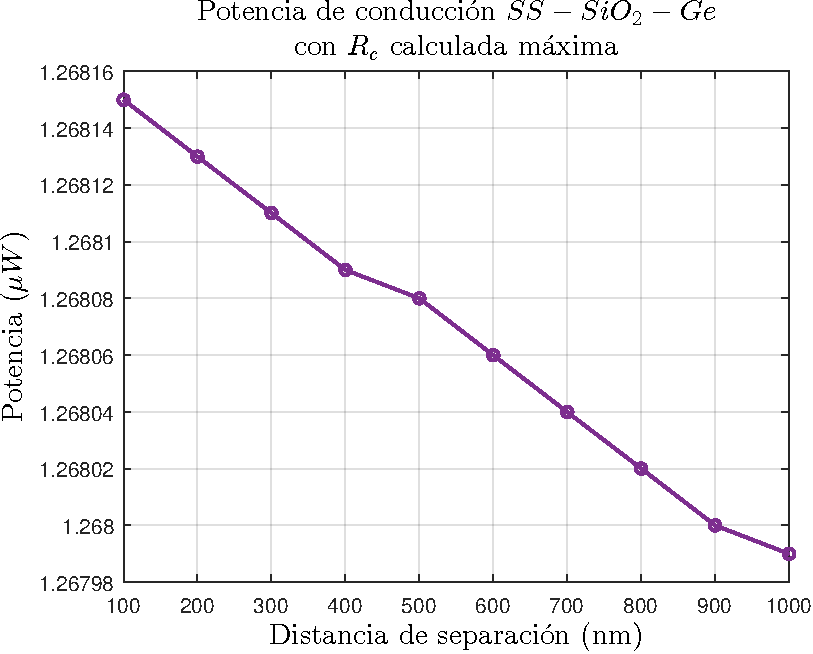
\includegraphics[width=1.00\textwidth]{Prc_SsSiO2Ge_Max.pdf}
		\caption{ }
		\label{fig:Prc_SsSiO2Ge_Max}
	\end{subfigure}
	\caption{Potencias por conducción para una nTPV $SS-SiO_2-Ge$ con $R_c$ calculadas a partir de las conductancias térmicas \cite{experimental_Rc_SS}, para una $R_c$ máxima de  $5.5\cdot 10^{-3} \ m^2 K/W$ (\subref{fig:Prc_SsSiO2Ge_Max}) y una $R_c$ intermedia $2.75\cdot 10^{-3} \ m^2 K/W$ (\subref{fig:Prc_SsSiO2Ge_Inter}) frente a las alturas de un nano-espaciadores.}
	\label{fig:Pcond1_SsSiO2Ge}
\end{figure}
Las potencias para las nTPV con $R_c$ calculadas son del orden de $\mu W$, y como se pueden observar en las figuras \ref{fig:Pcond1_SsSiO2Ge} (\subref{fig:Prc_SsSiO2Ge_Inter}) y (\subref{fig:Prc_SsSiO2Ge_Max}) las potencias son aproximadamente rectas con muy poca variación entre cada altura consecutiva de nano-espaciador, pudiéndose considerarse constantes para unos valores de $\sim 2.534 \mu W$ para la nTPV de $R_c$ calculada intermedia y $\sim 1.268 \mu W$ para la nTPV de $R_c$ calculada máxima.\\\\
Se calcula la relación de cada una de las potencias de conducción de las nTPV con $R_c$ respecto a la potencia conducida sin resistencia de contacto, obteniéndose una relación muy pequeña menos de un 0.03\% para las nTPVs con $R_c$ calculadas porque la resistencia total es mucho mayor que para la $R_c$ empírica, relación mínima de un 3\%.\\\\
Dado que la resistencia de contacto en las simulaciones es constante, no se procede a calcular un modelo analítico que relacione las potencias de conducción con las alturas de los nano-espaciadores y con la resistencia de contacto, y por la alta complejidad de la resistencia de contacto en la realidad, es decir, su alta dependencia en varios parámetros como la presión, temperatura, conductividades de los materiales, entre otros.
%%%   CAMPO CERCANO    SS
\subsection{Radiación de campo cercano}
Para la simulación de radiación de campo cercano solo se considera los resultados en el rango espectral de energía mayor a 0.7eV o longitud de onda de $\sim$1.8 $\mu m$ porque los datos de el índice de refracción $n$ y coeficiente de extinción $k$ del acero inoxidable llegan hasta los 1.2 $\mu m$ de longitud de onda \cite{ss_optical_2017}, realizando una extrapolación lineal hasta los 1.8$\mu m$ para poder obtener las potencias de radiación para diferentes distancias de separación.\\\\
Se comparan las potencias de radiación integradas en el rango espectral de energía mayor a 0.7eV para un emisor de Hierro ($Fe$) y de acero inoxidable para verificar que no existan grandes diferencias entre las potencias para un emisor de $SS$ respecto a las del $Fe$ como consecuencia de la extrapolación de los valores de $n$ y $k$ hasta los 1.8$\mu m$, se compara respecto al $Fe$ porque es el elemento principal que componena  los aceros.
\begin{figure}[H]
	\centering
		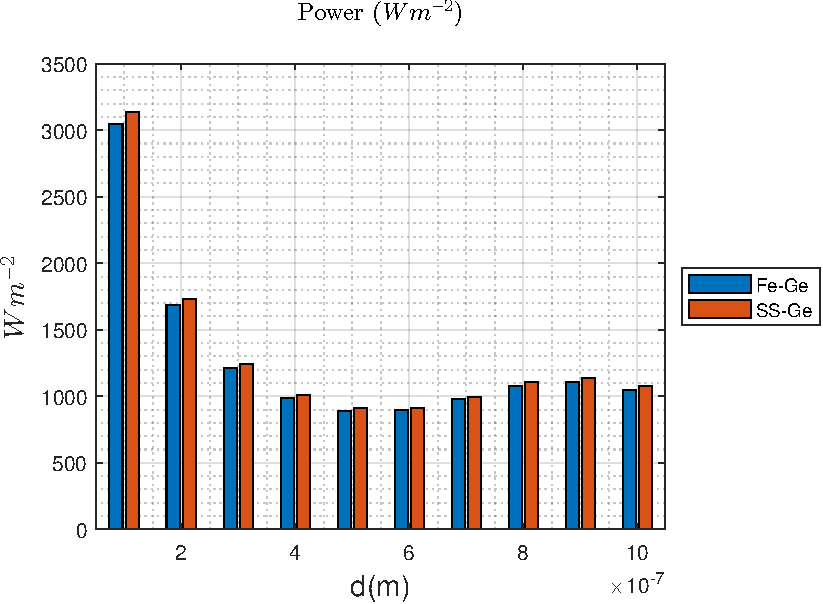
\includegraphics[width=0.65\textwidth]{figuras/rad_mat/FevsSs.pdf}
	\caption{Potencias por radiación integradas en el rango espectral de energía mayor a 0.7eV para un emisor de $Fe$ y un emisor de $SS$ con receptor de $Ge$ frente a las diferentes distancias de separación de las placas.}
	\label{fig:FevsSs}
\end{figure}
Se obtienen valores similares para todo el rango de distancias de separación estudiadas (figura \ref{fig:FevsSs}), de 100nm a 1000nm. Por lo tanto, se utiliza para las simulaciones de radiación de campo cercano el emisor de $SS$ con $n$ y $k$ extrapolados linealmente.\\\\
Se procede a simular la radiación por campo cercano para solo un emisor de $SS$ (figura \ref{fig:SsGe}), obteniéndose una potencia radiativa monocromática máxima menor que para el emisor de $Si$ (figura \ref{fig:rad_SiGe}) y también las potencias integradas en el rango espectral de energía superior a 0.7eV del emisor $SS$ (figura \ref{fig:p_Eg_SsGe}) son menores que para las del emisor de $Si$ (figura \ref{fig:p_Eg_SiGe}) para todas las distancias de separación.
\begin{figure}[H]
	\centering
	\begin{subfigure}[b]{0.49\textwidth}
	\centering
		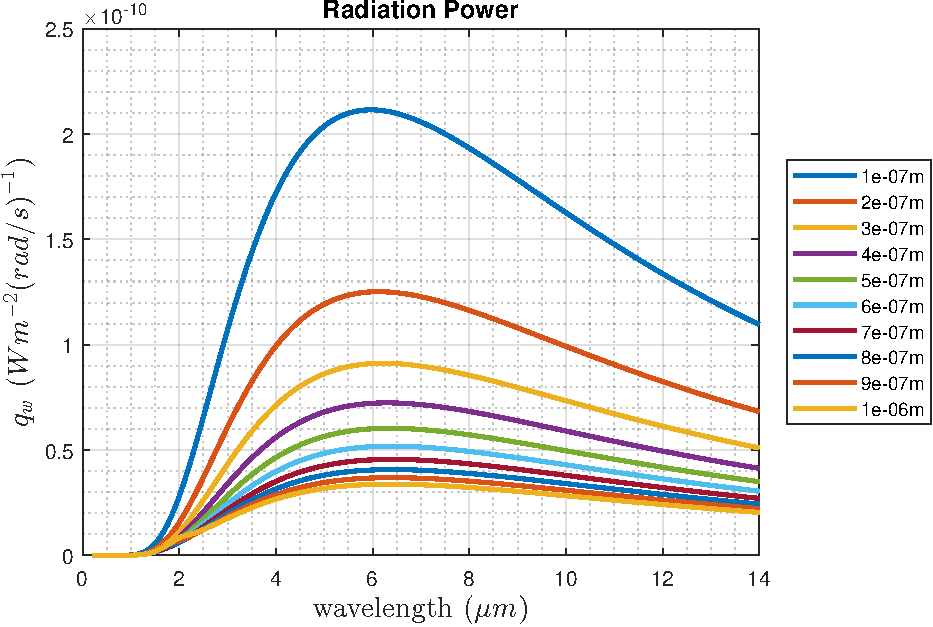
\includegraphics[width=1.00\textwidth]{figuras/Resultados/radiacion/SsGe.pdf}
	\caption{Potencia monocromática}
	\label{fig:SsGe}
\end{subfigure}
\begin{subfigure}[b]{0.49\textwidth}
	\centering
		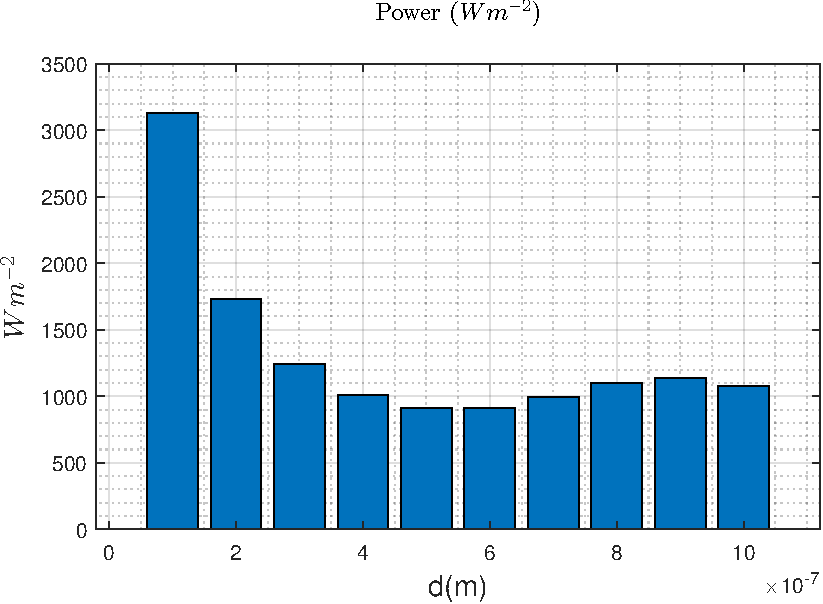
\includegraphics[width=1.00\textwidth]{figuras/Resultados/radiacion/p_Eg_SsGe.pdf}
	\caption{Potencia hasta 0.7 eV}
	\label{fig:p_Eg_SsGe}
\end{subfigure}
\caption{(\subref{fig:SsGe}) Potencia radiada monocromática por campo cercano para un emisor de $SS$ y una célula de $Ge$. (\subref{fig:p_Eg_SsGe}) Potencia radiada para un rango de longitudes de onda cuya energía es mayor a los 0.7eV ($\sim 1.8 \ \mu m$).}
	\label{fig:rad_SsGe}
\end{figure}
Las potencias integradas no son todas mayores de 1000 $Wm^{-2}$ para las distancias de separación de 500nm, 600nm y 700nm, pero en promedio se pueden considerar que las potencias se encuentran en el rango de los miles de $Wm^{-2}$ desde los 300nm a los 1000nm, creciendo en mayor proporción a partir de los 200nm hasta los 100nm.
%%%   DENSIDAD DE NANO-ESPACIADORES
\subsection{Densidad de nano-espaciadores}
Se realizan los cálculos de las densidades de nano-espaciadores para las relaciones de las potencias de radiación respecto a las de conducción para valores superiores por un orden de magnitud para los casos con $R_c$ y superiores a 3 para el caso sin $R_c$.
\begin{figure}[H]
	\centering
	\begin{subfigure}[b]{0.49\textwidth}
		\centering
			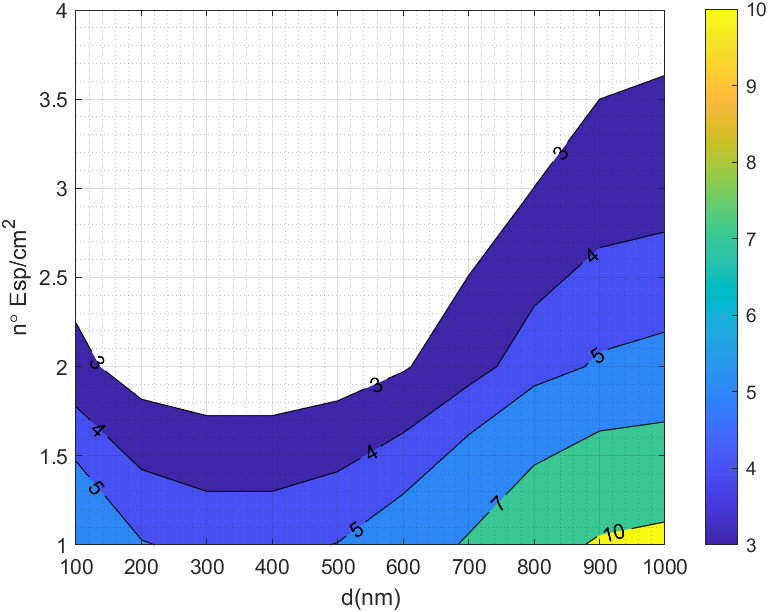
\includegraphics[width=1.00\textwidth]{figuras/Resultados/RelacionCondRad/SS.png}
		\caption{Sin $R_c$}
		\label{fig:rel_SsSiO2Ge}
	\end{subfigure}
	\hfill
	\begin{subfigure}[b]{0.49\textwidth}
		\centering
			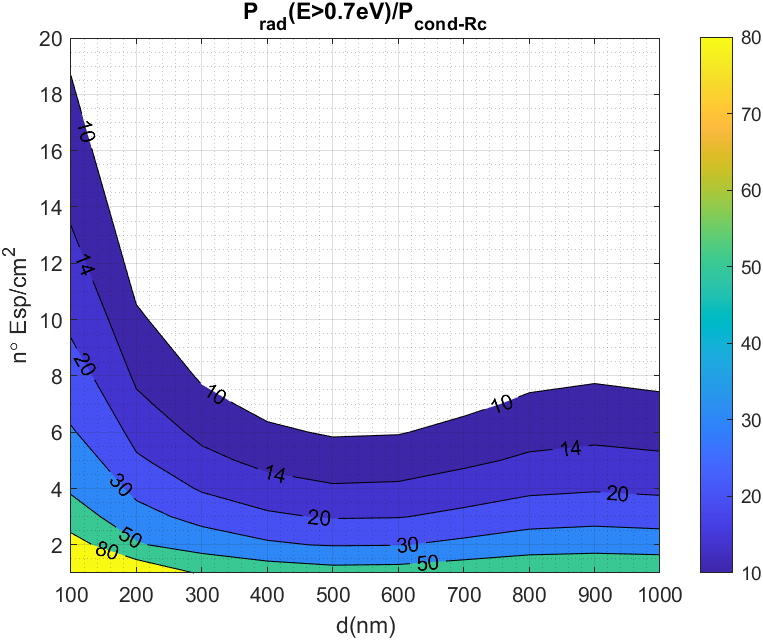
\includegraphics[width=1.00\textwidth]{figuras/Resultados/RelacionCondRad/SS_Rc_empirico.png}
		\caption{$R_c$ empírica}
		\label{fig:rel_SsSiO2Ge_Rc_emp}
	\end{subfigure}
	\caption{Densidades de nano-espaciadores para todas las relaciones de las potencias de radiación respecto a las conducción para un emisor de $SS$ frente a las altura de los nano-espaciadores para un emisor y una célula de 1 $cm^2$ sin $R_c$ (\subref{fig:rel_SsSiO2Ge}) y con $R_c$ empírica (\subref{fig:rel_SsSiO2Ge_Rc_emp}). El espectro de colores para cada relación entre las potencias de cada gráfica está indicado en las barra de colores lateral en el rango de valores que se encuentran en los extremos de cada barra.}
	\label{fig:rels_SsSiO2Ge_PnvsRc}
\end{figure}
Las densidades de nano-espaciadores obtenidas son menores que para la nTPV de $Si-SiO_2-Ge$ para todas las relaciones de potencias, siendo para el caso sin $R_c$ entre 1 a 2 nano-espaciadores menos por $cm^2$. Para las densidades de las nTPVs con $R_c$ para una altura de nano-espaciadores de 100nm la densidad disminuye de unos $\sim$30 $n^{\circ} esp/cm^2$ (figura \ref{fig:rel_SiSiO2Ge_Rc}) para la nTPV de $Si-SiO_2-Ge$ a unos $\sim$19 $n^{\circ} esp/cm^2$ (figura \ref{fig:rel_SsSiO2Ge_Rc_emp}) para la nTPV de $SS-SiO_2-Ge$ porque la potencia radiada es menor para el emisor de $SS$ que para el emisor de $Si$.
\begin{figure}[H]
	\centering
	\begin{subfigure}[b]{0.49\textwidth}
		\centering
			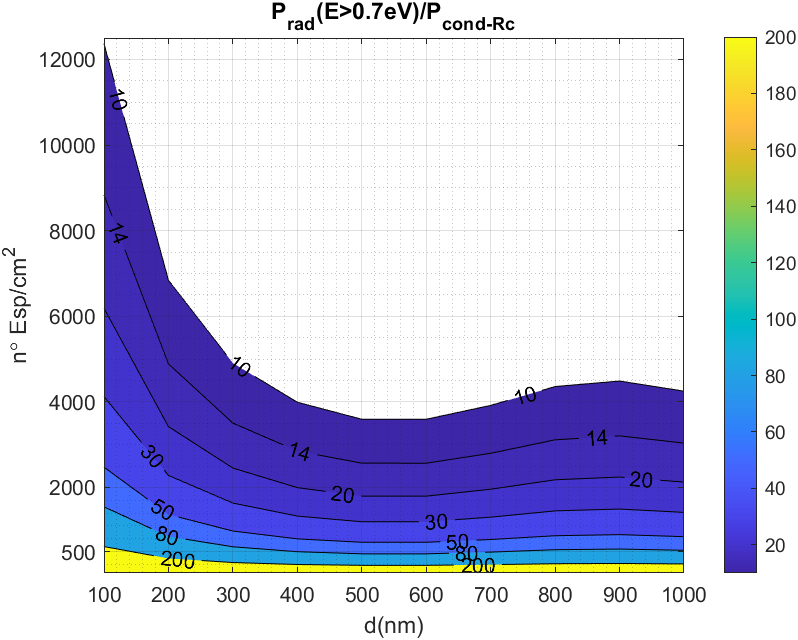
\includegraphics[width=1.00\textwidth]{figuras/Resultados/RelacionCondRad/SS_Rc_Intermedio.png}
		\caption{$R_c$ calculada intermedia}
		\label{fig:rel_SsSiO2Ge_Rc_inter}
	\end{subfigure}
	\hfill	
	\begin{subfigure}[b]{0.49\textwidth}
		\centering
			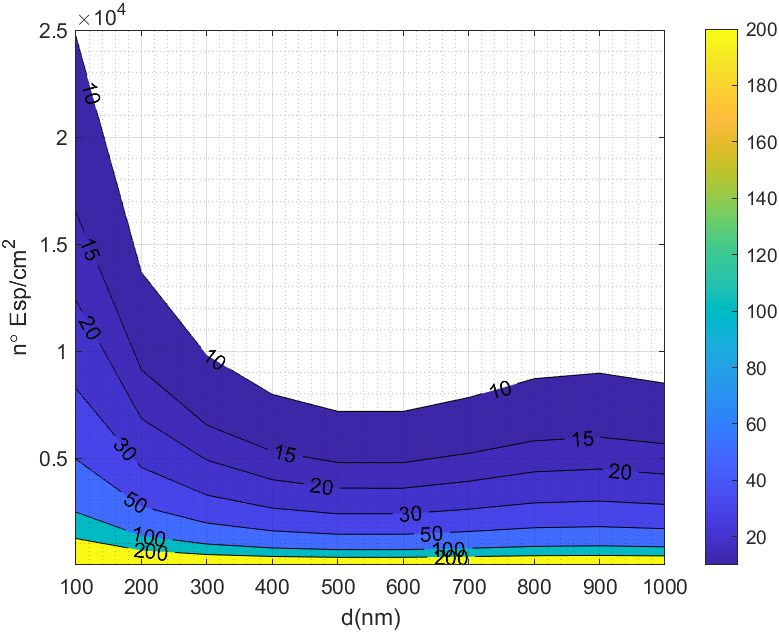
\includegraphics[width=1.00\textwidth]{figuras/Resultados/RelacionCondRad/SS_Rc.png}
		\caption{$R_c$ calculada máxima}
		\label{fig:rel_SsSiO2Ge_Rc_max}
	\end{subfigure}
	\caption{Densidades de nano-espaciadores para todas las relaciones de las potencias de radiación respecto a las conducción para un emisor de $SS$ frente a las altura de los nano-espaciadores para un emisor y una célula de 1 $cm^2$ con $R_c$ calculada intermedia (\subref{fig:rel_SsSiO2Ge_Rc_inter}) y con $R_c$ calculada máxima (\subref{fig:rel_SsSiO2Ge_Rc_max}). El espectro de colores para cada relación entre las potencias de cada gráfica está indicado en las barra de colores lateral en el rango de valores que se encuentran en los extremos de cada barra.}
	\label{fig:rels_SsSiO2Ge_Prc1vsPrc2}
\end{figure}
Para los casos con $R_c$ calculadas, las densidades de nano-espaciadores para una relación mínima de potencias de un orden de magnitud son del orden de $10^4 \ n^{\circ}esp/cm^2$ y disminuyendo al orden de los miles de $n^{\circ}esp/cm^2$ para relaciones de potencias de dos ordenes de magnitud. Para las relaciones de las potencias de dos ordenes de magnitud las densidades de nano-espaciadores a una altura de nano-espaciadores de 100nm son $\sim$ 2500 $n^{\circ} esp/cm^2$ para la nTPV con $R_c$ intermedia y $\sim$ 1000 $n^{\circ} esp/cm^2$ para la nTPV con $R_c$ máxima (figuras \ref{fig:rels_SsSiO2Ge_Prc1vsPrc2} \subref{fig:rel_SsSiO2Ge_Rc_inter} y \subref{fig:rel_SsSiO2Ge_Rc_max}).\\\\
Se observa que la relación entre las densidades de nano-espaciadores para ambos casos de $R_c$ calculada es aproximadamente igual a la relación entre ambas resistencias de contacto porque son constantes y solo afectan a la conducción en las simulaciones. El conocer estas relaciones es de utilidad para poder determinar en una primera instancia que valor de resistencia de contacto sería necesario como mínimo para tener la relación de potencias deseada con una cierta cantidad de nano-espaciadores de cierta altura.\\\\
También es importante tener en cuenta la variación de la densidad de nano-espaciadores o de la potencia de radiación entre su valor máximo y mínimo para una relación de potencias de un orden de magnitud porque las superficies tanto del emisor como de la célula presentan curvaturas que provocan un aumento o disminución de las distancias de separación entre ambos componentes, por ende, un aumento o disminución de las potencias de radiación útiles para su conversión en electridad.\\\\
Se realizan los cálculos del peor caso de estas variaciones, cuando la densidad va de su valor máximo a su valor mínimo. Para el caso con $R_c$ empírica la variación de las densidades  es de aproximadamente 12 $n^{\circ} esp/cm^2$ que representa una disminución del 66.67\% respecto al valor pico, para el caso con $R_c$ calculada intermedia la variación es de $\sim$8500 $n^{\circ} esp/cm^2$  que es una disminución del 70.83\% y para el caso de $R_c$ calculada máxima la variación de densidad es aproximadamente unos 18$\cdot 10^3 \ n^{\circ}esp/cm^2$ que es una disminución del 72\%. Aunque al aumentar la $R_c$ aumenta la disminución porcentual de las densidades, no es algo tan importante mientras la densidad de nano-espaciadores es lo suficientemente alta para poder mantener mejor la separación entre ambas placas manteniendo una relación de potencias de producción vs pérdidas alta, es decir, la relación entre las potencias sea al menos de un orden de magnitud.\\\\
Por último, se recopilan los resultados obtenidos de las simulaciones en la tabla \ref{tab:SsSiO2Ge} para tener una mejor idea de los valores numéricos y de la magnitud de los resultados.
\begin{table}[H]
	\centering
		\begin{tabular}{|c||c|c|c|c||c|}
		\hline
		\multirow{2}{*}{ }& \multicolumn{5}{c|}{\textbf{\large Potencias según transmisión del calor}}\\ \cline{2-6}
& \multicolumn{4}{c||}{Conducción (W/nº esp.)}& Radiación $(W/m^2)$\\ \hline
Dist. (nm)&$P_{Normal}$&$P_{R_c-Cal.Max}$&$P_{R_c-Cal.Inter}$&$P_{R_c-Empirico}$&$P_{Eg>0.7eV}$\\ \hline \hline
100&4,80E-02&1,26815E-06&2,53438E-06&1,68E-03&3,13E+03\\ \hline 
200&3,42E-02&1,26813E-06&2,53431E-06&1,65E-03&1,73E+03\\ \hline 
300&2,64E-02&1,26811E-06&2,53424E-06&1,62E-03&1,24E+03\\ \hline 
400&2,15E-02&1,26809E-06&2,53417E-06&1,60E-03&1,01E+03\\ \hline 
500&1,81E-02&1,26808E-06&2,53410E-06&1,57E-03&9,11E+02\\ \hline 
600&1,56E-02&1,26806E-06&2,53403E-06&1,54E-03&9,10E+02\\ \hline 
700&1,37E-02&1,26804E-06&2,53396E-06&1,52E-03&9,93E+02\\ \hline 
800&1,22E-02&1,26802E-06&2,53388E-06&1,50E-03&1,10E+03\\ \hline 
900&1,11E-02&1,26800E-06&2,53381E-06&1,48E-03&1,14E+03\\ \hline 
1000&1,01E-02&1,26799E-06&2,53374E-06&1,45E-03&1,08E+03\\ \hline 
		\end{tabular}
	\caption{Tabla de recopilación de los resultados de las simulaciones de transmisión de calor por conducción y radiación de campo cercano para una nTPV de emisor de $SS$.}
	\label{tab:SsSiO2Ge}
\end{table}
\vfill \newpage
%%%%%%%%%%%    SiC-SiO2-Ge
\section{Resultados de las simulaciones para una nTPV de SiC-SiO2-Ge}\label{sec:res_SiCSiO2Ge}
Se procede a estudiar el caso de una nTPV con un emisor de Carburo de Silicio ($SiC$) por ser una material con mayor conductividad térmica que el $Si$ y el $SS$ a 800\textdegree C, que rondan unos 60 $W/(m^2 K)$ para el emisor de $SiC$, 26 $W/(m^2 K)$ para el $Si$ y 30 $W/(m^2 K)$ para el $SS$. Además el $SiC$ tiene un punto de fusión mayor que el $Si$ y el $SS$, siendo una característica del material de gran utilidad para su uso en baterías para almacenar la energía en forma de calor.\\\\
Otra razón de estudiar la nTPV con emisor de $SiC$ es por su utilización en \cite{doi:Near_field_ThinFilm} en una capa fina depositada sobre el emisor de una nTPV para aumentar el flujo de calor por radiación de campo cercano simulado entre el emisor y el receptor de $SiC$ grueso.
%%%%%    CFD
\subsection{Simulaciones de CFD}
\graphicspath{ {./figuras/Resultados/conduccion/pdf/} }
\begin{figure}[H]
	\centering
	\begin{subfigure}[b]{0.49\textwidth}
		\centering
			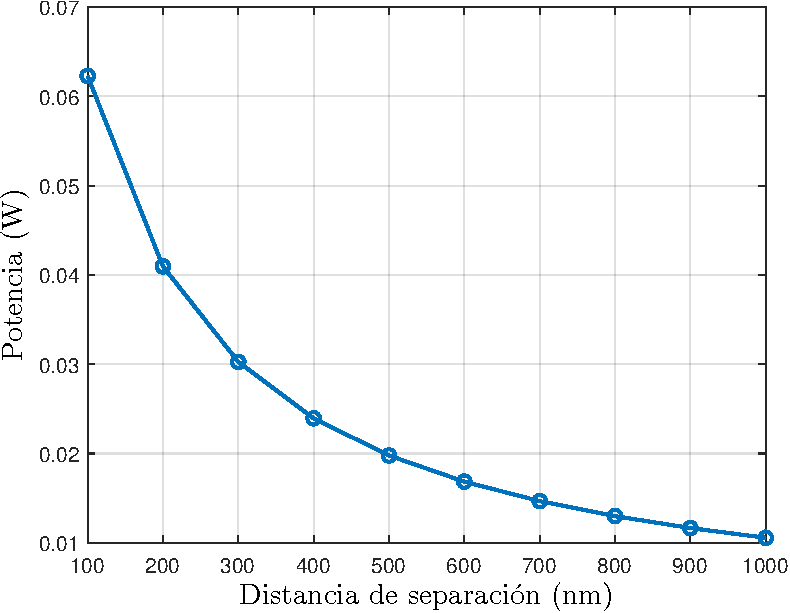
\includegraphics[width=1.00\textwidth]{Pn_SiCSiO2Ge.pdf}
		\caption{Potencias de conducción}
		\label{fig:Prc_SiCSiO2Ge}
	\end{subfigure}
	\hfill
	\begin{subfigure}[b]{0.49\textwidth}
		\centering
			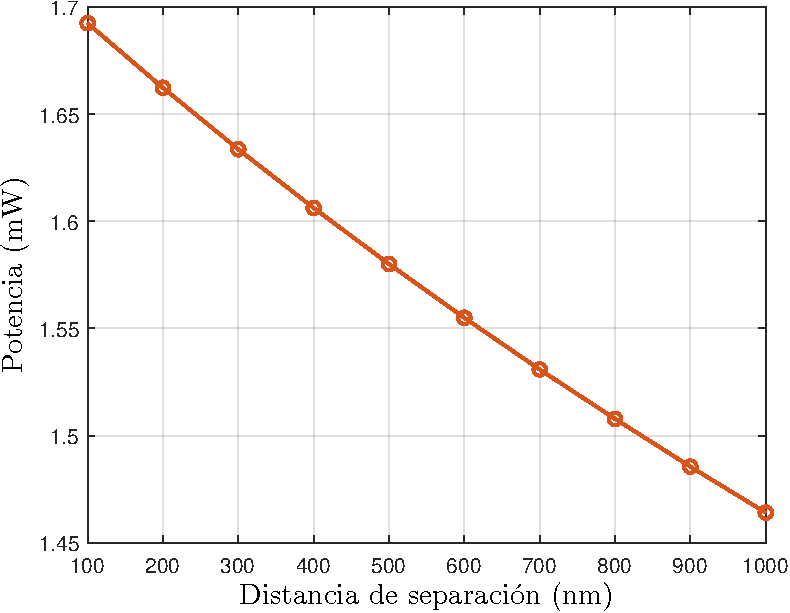
\includegraphics[width=1.00\textwidth]{Prc_SiCSiO2Ge.pdf}
		\caption{Relación de potencia $R_c$}
		\label{fig:relPrc_SiCSiO2Ge}
	\end{subfigure}
	\caption{(\subref{fig:Prc_SiCSiO2Ge}) Potencias de conducción para sin y con el efecto de la $R_c$ empírica, eje izquierdo para el caso sin $R_c$ y eje derecho para el caso con $R_c$. (\subref{fig:relPrc_SiCSiO2Ge}) Relación de la potencia de conducción con $R_c$ respecto a sin $R_c$.}
	\label{fig:PrcCond_SiCSiO2Ge}
\end{figure}
Se realizan las simulaciones de transmisión de calor por conducción, obteniéndose resultados similares a los casos anteriores porque la mayor cantidad de caída de temperatura se produce en el nano-espaciador por tener una baja conductividad térmica respecto al emisor y la célula. Algo que si se nota es que la potencia máxima es $\sim 0.85\cdot 10^{-2}$ W mayor que para el emisor de $Si$ pero la relación entre las potencias con $R_c$ respecto a sin $R_c$ es menor, no superando el 14\% como valor máximo a los 1000nm.\\\\
\subsection{Radiación de campo cercano}
Se realizan las simulaciones de transmisión de calor por radiación de campo cercano para el emisor de $SiC$, obteniéndose valores de potencia radiada monocromática similares al del emisor de $Si$ para longitudes de onda menores a 2$\mu m$ (figura \ref{fig:rad_SiCGe}) y también tiene valores similares de la potencia radiada integrada en el rango espectral de energía mayor a 0.7eV frente a las distancias de separación respecto al emisor de $Si$ (figura \ref{fig:Prad_SiCGe}).
%%%           GRAFICAS
\graphicspath{ {./figuras/Resultados/radiacion} }
\begin{figure}[H]
	\centering
	\begin{subfigure}[b]{0.49\textwidth}
		\centering
		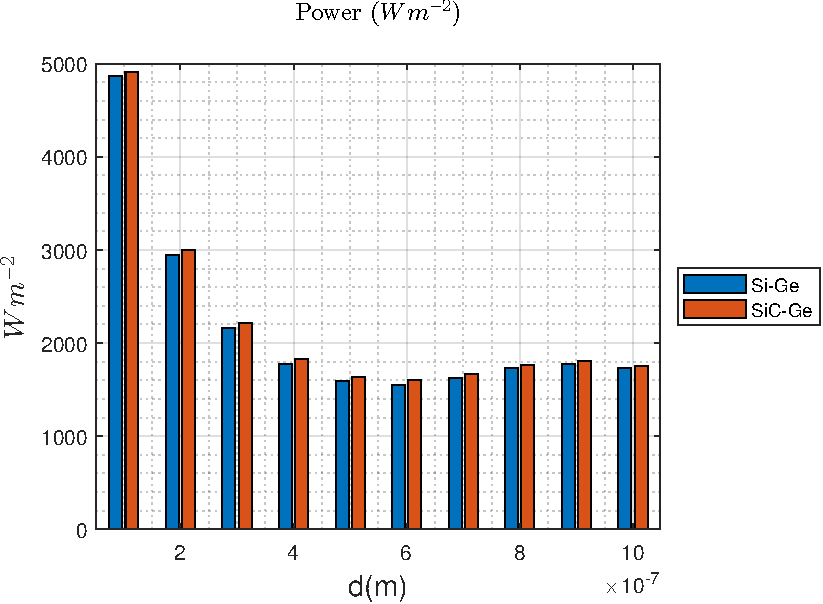
\includegraphics[width=1.00\textwidth]{SiCvsSi.pdf}
		\caption{Potencia integrada}
		\label{fig:Prad_SiCGe}
	\end{subfigure}
	\hfill
	\begin{subfigure}[b]{0.49\textwidth}
		\centering
		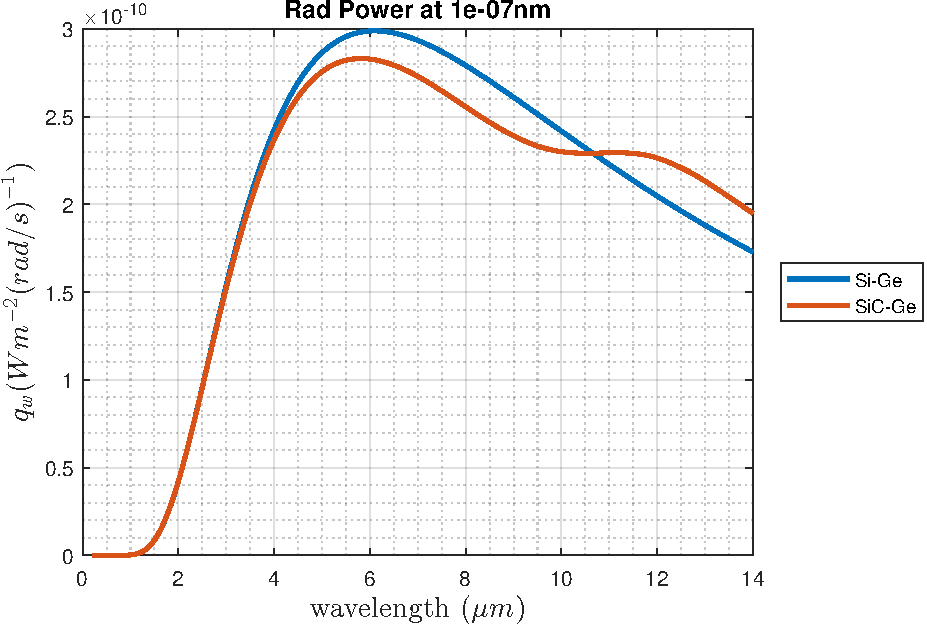
\includegraphics[width=1.00\textwidth]{SiCvsSi_rad.pdf}
		\caption{Radiación}
		\label{fig:rad_SiCGe}
	\end{subfigure}
	\caption{(\subref{fig:Prad_SiCGe}) Potencias integradas en el rango espectral de energía mayor a 0.7eV para un emisor de $SiC$ y un emisor de $Si$ frente a las distancias de separación entre emisor y receptor. (\subref{fig:rad_SiCGe}) Potencia de radiación monocromática para un emisor de $Si$ y $SiC$ con un receptor de $Ge$ para una distancia de separación de 100nm frente longitudes de onda.}
	\label{fig:rads_SiCGe}
\end{figure}
Aunque las potencias radiadas monocromáticas, es decir, frente a las longitudes de onda, difieren al aumentar la longitud de onda ($\lambda$), no supone una gran diferencia entre ambos emisores porque en el rango energético de interés ($E>0.7eV$) las curvas son bastante similares, provocando que las potencias integradas en dicho rango energético sean similares también.
\begin{figure}[H]
	\centering
		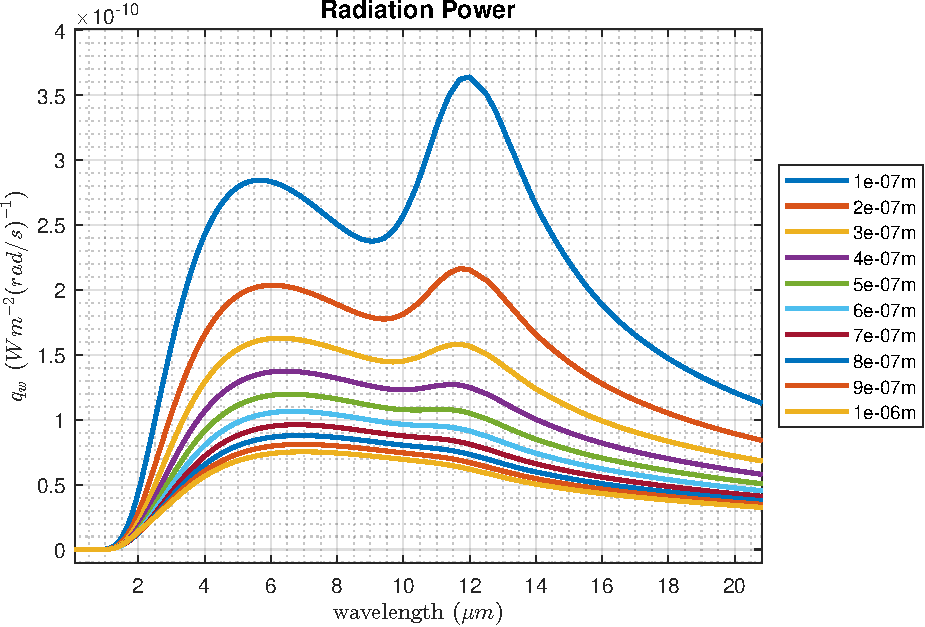
\includegraphics[width=0.65\textwidth]{figuras/Resultados/radiacion/SiCSiC.pdf}
	\caption{Potencias de radiación monocromática frente a las longitudes de onda para un sistema de $SiC-SiC$ frente a diferentes distancias de separación entre placas.}
	\label{fig:SiCSiC}
\end{figure}
También se simula un sistema con receptor de $SiC$ y emisor de $SiC$ para observar los efectos de la frecuencia de resonancia ($\omega_{res}$) sobre las potencias de radiación frente a las longitudes de onda. Se observa en la figura \ref{fig:SiCSiC} que la $\omega_{res}$ es aproximadamente $1.57\cdot 10^{14} \ rad/s$ ($\lambda = 12\mu m$) porque existe un pico de potencia monocromática máxima que disminuye al aumentar la distancia de separación entre emisor y receptor, pudiéndose aprovechar dicha potencia para la conversión en electricidad si mediante una combinación de materiales se consigue que la frecuencia se encuentre dentro del rango espectral útil.
%%%    DENSIDAD
\subsection{Densidad de nano-espaciadores}
Se procede a calcular las densidades de nano-espaciadores por centímetro cuadrado para la nTPV con emisor de $SiC$ para los casos de sin $R_c$ y con $R_c$ de $4\cdot 10^{-6} \ m^2 K/W$ \cite{nf_TPV_Pillars_SiO2}. Obteniéndose unos resultados muy parecidos a los de la nTPV de emisor de $Si$ porque los resultados obtenidos de las simulaciones también son bastante cercanos.
\graphicspath{ {./figuras/Resultados/RelacionCondRad} }
\begin{figure}[H]
	\centering
	%% Si-SiO2-Si Eg
	\begin{subfigure}[b]{0.49\textwidth}
		\centering
		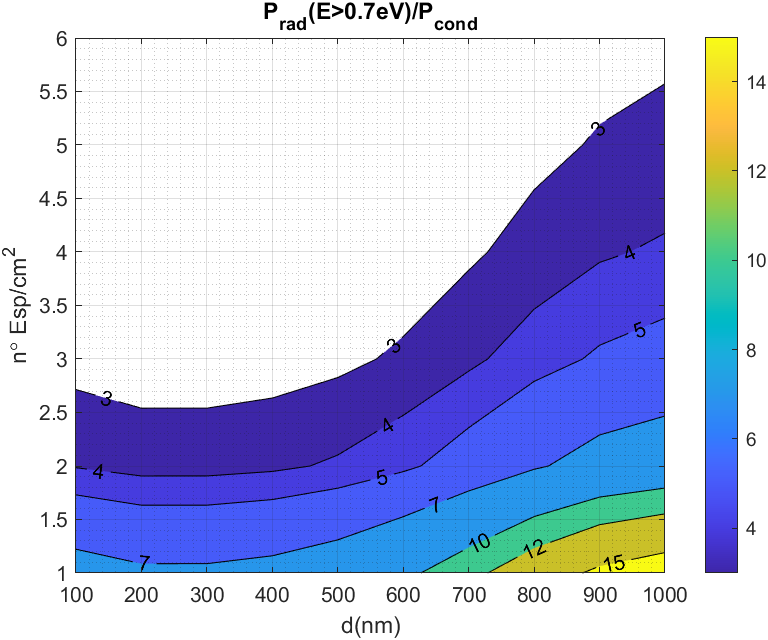
\includegraphics[width=1.00\textwidth]{SiC_Ge.png}
		\caption{ }
		\label{fig:rel_SiCSiO2Ge}
	\end{subfigure}
	\hfill
	\begin{subfigure}[b]{0.49\textwidth}
		\centering
		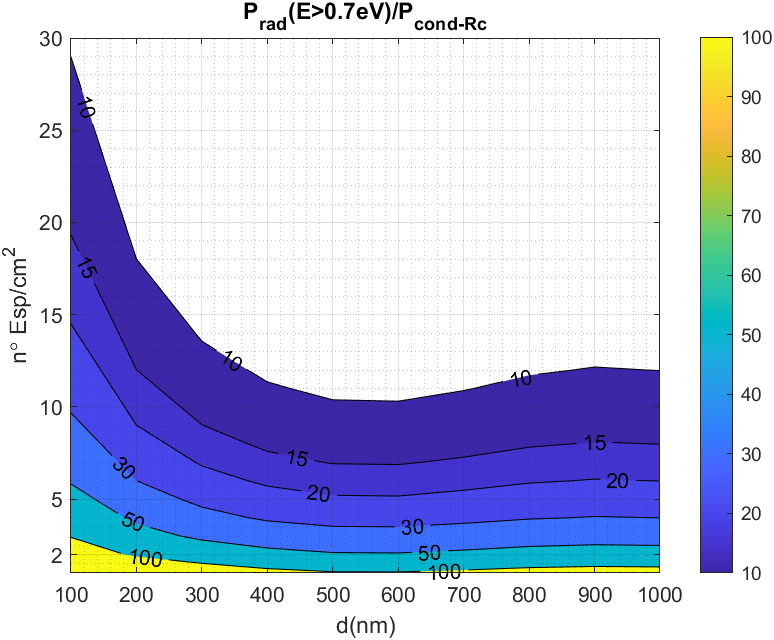
\includegraphics[width=1.00\textwidth]{SiC_Rc.png}
		\caption{ }
		\label{fig:rel_SiCSiO2Ge_Rc}
	\end{subfigure}
	\caption{Densidades de nano-espaciadores ($n^{\circ}esp/cm^2$) frente a las alturas de los nano-espaciadores para todas las relaciones de la potencia de radiación en el rango espectral de energías mayores e igual a 0.7 eV respecto a las potencias de conducción (dependientes en la densidad de nano-espaciadores) mayores a 3 para el caso sin $R_c$ (\subref{fig:rel_SiCSiO2Ge}) y mayores a 10 para el caso con $R_c$ (\subref{fig:rel_SiCSiO2Ge_Rc}). Donde las barras de colores laterales de cada gráfica representan los colores asociados a cada uno de los valores de las relaciones de las potencias, con los contornos de las relaciones más significativas representadas en las gráficas.}
	\label{fig:relation_SiCSiO2Ge}
\end{figure}
La principal diferencia es en las densidades de nano-espaciadores para el caso de la nTPV sin $R_c$ (figura \ref{fig:rel_SiCSiO2Ge}), siendo esta menor que la del emisor de $Si$ para todo el rango de alturas de los nano-espaciadores porque la conductividad térmica del $SiC$ a 800\textdegree C es mayor que para el $Si$ por lo tanto la resistencia térmica del sistema disminuye, teniendo así unas menores densidades. Para el caso de la nTPV con $R_c$, las diferencias no son tan notables como en el caso sin $R_c$ porque la componente con mayor relevancia es la resistencia de contacto.\\\\
Por último, se recopilan los resultados obtenidos de las simulaciones de transferencia de calor por conducción y radiación de campo cercano en la tabla \ref{tab:SiCSiO2Ge}, los resultados se muestran en notación científica para simplificar el análisis de los mismos.
\begin{table}[h]
	\centering
		\begin{tabular}{|c||c|c||c|c|}
		\hline
\multirow{2}{*}{ }& \multicolumn{4}{c|}{\textbf{\large Potencias según transmisión del calor}}\\ \cline{2-5}
& \multicolumn{2}{c||}{Conducción (W/nº esp.)}& \multicolumn{2}{c|}{Radiación $(W/m^2)$}\\ \hline
Dist. (nm)&$P_{Normal}$&$P_{R_c-Empirico}$&$P_{Eg>0.7eV}$&$P_{full}$\\ \hline \hline
100&6,23E-02&1,69E-03&4,90E+03&1,50E+05\\ \hline 
200&4,09E-02&1,66E-03&3,00E+03&1,01E+05\\ \hline 
300&3,03E-02&1,63E-03&2,21E+03&7,80E+04\\ \hline 
400&2,39E-02&1,61E-03&1,82E+03&6,43E+04\\ \hline 
500&1,98E-02&1,58E-03&1,64E+03&5,52E+04\\ \hline 
600&1,68E-02&1,55E-03&1,60E+03&4,87E+04\\ \hline 
700&1,47E-02&1,53E-03&1,67E+03&4,40E+04\\ \hline 
800&1,30E-02&1,51E-03&1,76E+03&4,06E+04\\ \hline 
900&1,17E-02&1,49E-03&1,81E+03&3,80E+04\\ \hline 
1000&1,06E-02&1,46E-03&1,75E+03&3,61E+04\\ \hline 
		\end{tabular}
	\caption{Tabla de recopilación de los resultados de las simulaciones de transmisión de calor por conducción y radiación de campo cercano para una nTPV de emisor de $SS$.}
	\label{tab:SiCSiO2Ge}
\end{table}

\vfill \newpage
%%%     NUMERO DE NANO-ESPACIADORES
\section{Densidad de nano-espaciadores para soportar la carga}\label{sec:densidad_carga}
Dado que los nano-espaciadores tendrán que soportar el peso del emisor o la célula se estudia la cantidad mínima de nano-espaciadores necesarios en un centímetro cuadrados para soportar la carga. También se estudia la densidad de nano-espaciadores para el caso de que se aplique una presión de una atmósfera a una de las caras para asegurar que las distancias de separación sean lo más uniformes posibles.\\\\
La fuerza de compresión del $SiO_2$ es de unos $1.68 \ MPa$ y la densidad mayor entre los materiales de emisor y células es el acero inoxidable 304, con una densidad aproximada de $8 \ g/cm^3$ o $8\cdot 10^3 kg/m^3$. Para un emisor $SS$ de área $1 \ cm^2$ y espesor de $0.5 \ cm$ la masa total es de unos 4 $gr$ o un peso de unos $\sim 0.04 \ N$, obteniéndose una densidad mínima de nano-espaciadores para solo soportar la carga del emisor de $3 \ n^{\circ}esp/cm^2$, un valor bastante pequeño para disminuir las curvaturas por flexión o imperfecciones del acabado de la superficie del emisor, pero teniendo una mayor relación entre las potencias de radiación respecto a las de conducción, es decir, mayor transferencia de potencia útil respecto a las pérdidas por conducción, disminuyendo así el aumento indeseado de la temperatura de la célula.\\\\
Al aplicarse una presión de una atmósfera sobre la superficie superior del emisor de la nTPV, la fuerza que soportan los nano-espaciadores aumenta hasta los $10.17 \ N$ generando que se necesiten una densidad mínima de nano-espaciadores de $673 \ n^{\circ}esp/cm^2$ para poder soportar la carga. Está densidad mínima es bastante alta respecto a las obtenidas en todos los casos de nTPVs de célula de germanio estudiados con resistencia de contacto empírica de $4\cdot 10^{-6} \ m^2 K/W$, pero no es tan elevada para el caso de la nTPV $SS-SiO_2-Ge$ con las $R_c$ calculadas para una relación de potencias mayor de un orden de magnitud (figuras \ref{fig:rels_SsSiO2Ge_Prc1vsPrc2} \subref{fig:rel_SsSiO2Ge_Rc_inter} y \subref{fig:rel_SsSiO2Ge_Rc_max}) porque sus valores de $R_c$ son mayores que la $R_c$ empírica y por ende, disminuyen las pérdidas que provoca un aumento de las densidades.
\vfill \newpage
%%    COMPARACION MATERIAL NANO-ESPACIADORES
\section{Resultados de las simulaciones para unas nTPVs de nano-espaciadores de Si}\label{sec:res_XxSiGe}
\graphicspath{ {./figuras/Resultados/DiffMatEsp} }
Como último caso de simulación se simula la transmisión de calor en CFD por conducción para una nTPV de nano-espaciador de $Si$ para un emisor de $Si$, un emisor de $SS$ y un emisor de $SiC$ con resistencias de contacto empíricas de $4\cdot 10^{-6} \ m^2 K/W$ porque durante el proceso de fabricación de la nTPV, específicamente la deposición del nano-espaciador, no se llegara a conseguir depositar $SiO_2$ sino $Si$.
%% comparar el efecto de cambiar el material del nano-espaciador
\begin{table}[H]
	\centering
		\begin{tabular}{|c||c|c|c|}
		\hline
		 \multicolumn{4}{|c|}{\textbf{Potencias de Conducción ($mW$)}}\\	\hline
		Dist. (nm)&$P_{R_c-Si}$&$P_{R_c-SS}$&$P_{R_cSiC}$\\ \hline \hline 
		100&$1.7136$&$1.7113$&$1.7261$\\ \hline 
		200&$1.7135$&$1.7112$&$1.7260$\\ \hline 
		300&$1.7134$&$1.7110$&$1.7258$\\ \hline 
		400&$1.7132$&$1.7109$&$1.7257$\\ \hline 
		500&$1.7130$&$1.7107$&$1.7255$\\ \hline 
		600&$1.7128$&$1.7105$&$1.7252$\\ \hline 
		700&$1.7126$&$1.7103$&$1.7250$\\ \hline 
		800&$1.7125$&$1.7102$&$1.7249$\\ \hline 
		900&$1.7122$&$1.7099$&$1.7246$\\ \hline 
		1000&$1.7121$&$1.7098$&$1.7244$\\ \hline
		\end{tabular}
	\caption{Tabla de recopilación de los resultados de las simulaciones de transferencia de calor por conducción para las nTPVs con nano-espaciador de Si y emisores de $Si$, $SS$ y $SiC$ respecto a cada altura del nano-espaciador.}
	\label{tab:nanoEspaciadorDeSi}
\end{table}
En primer lugar, de los resultados de las simulaciones de CFD, recopiladas en la tabla \ref{tab:nanoEspaciadorDeSi}, se observa como las pérdidas de conducción son mayores para los nano-espaciadores de $Si$ (figura \ref{fig:prc_xxSi}) que para los nano-espaciador de $SiO_2$ (figura \ref{fig:prc_xxSiO2}) porque la conductividad del $Si$ es mayor que la del $SiO_2$. Por lo tanto, la resistencia térmica del nano-espaciador es menos significativa y la resistencia de contacto tiene una mayor importancia.
\begin{figure} [H]%
	\centering
	\begin{subfigure}[b]{0.48\textwidth}%
			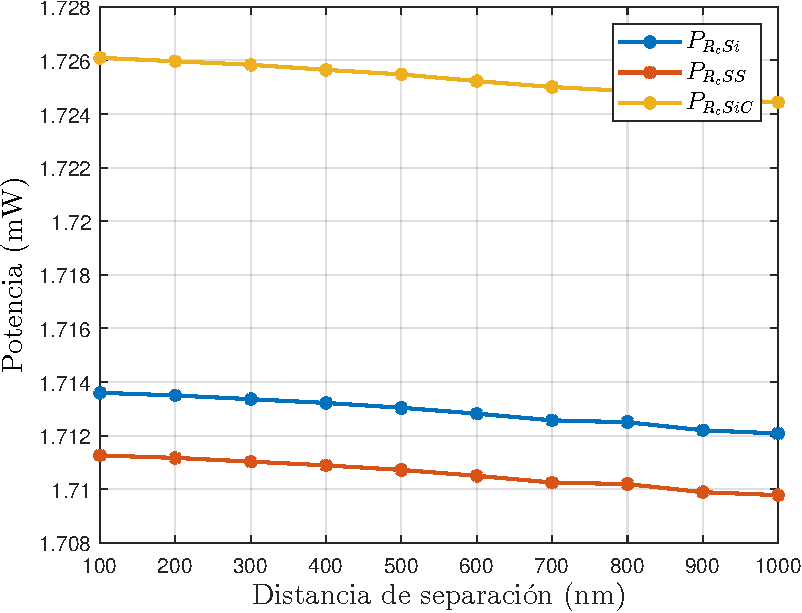
\includegraphics[width=\columnwidth]{Prc_XxSiGe}%
			\caption{}%
			\label{fig:prc_xxSi}%
	\end{subfigure}
	\hfill
	\begin{subfigure}[b]{0.48\textwidth}%
			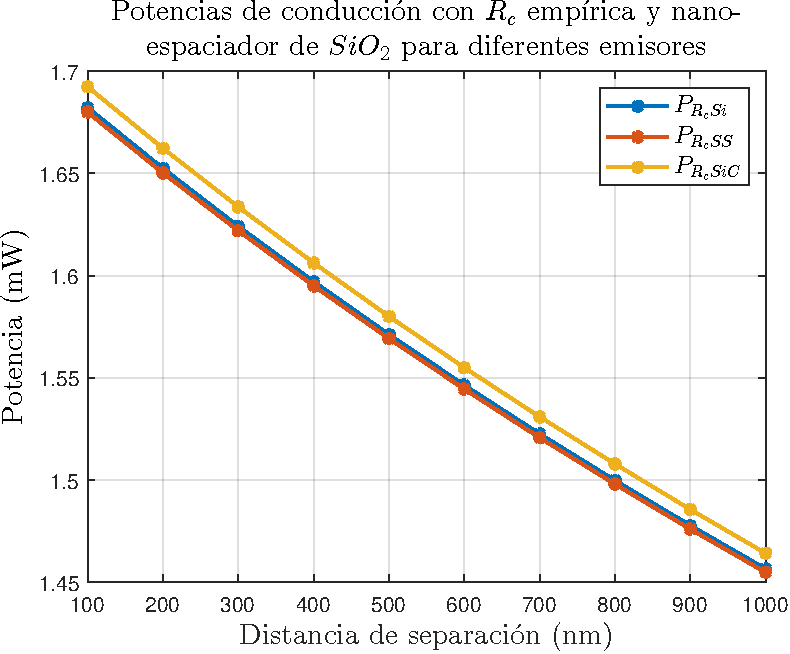
\includegraphics[width=\columnwidth]{Prc_XxSiO2Ge}%
			\caption{}%
			\label{fig:prc_xxSiO2}%
	\end{subfigure}
	\caption{Potencias de conducción de unas nTPVs con emisores de $Si$, $SS$ y $SiC$ frente a las alturas de un solo nano-espaciador en nanometros para un nano-espaciador de $Si$ (\subref{fig:prc_xxSi}) y para un nano-espaciador de $SiO_2$ (\subref{fig:prc_xxSiO2}).}%
	\label{fig:prc_xxXX}%
\end{figure}
En segundo lugar, se observa como las curvas de las potencias de conducción no varían tanto entre su valor máximo y valor mínimo, siendo para el caso de las nTPVs con nano-espaciadores de $Si$ el que presenta la menor variación de los dos, siendo esta menor de $0.002 \ mW$ (figura \ref{fig:prc_xxSi}), a diferencia de los nano-espaciadores de $SiO_2$ cuya variación es menor a los $0.25 \ mW$ (figura \ref{fig:prc_xxSiO2}). También se observa con mayor detalle como la diferencias de las resistencias de contacto de los materiales afecta al flujo de calor, aumentando con la disminución de la resistencia de contacto o aumento de la conductividad térmica, cuyos valores se mencionan en la sección \ref{sec:res_SiCSiO2Ge}.
\begin{figure} [H]%
	\centering
	\begin{subfigure}[b]{0.48\textwidth}%
			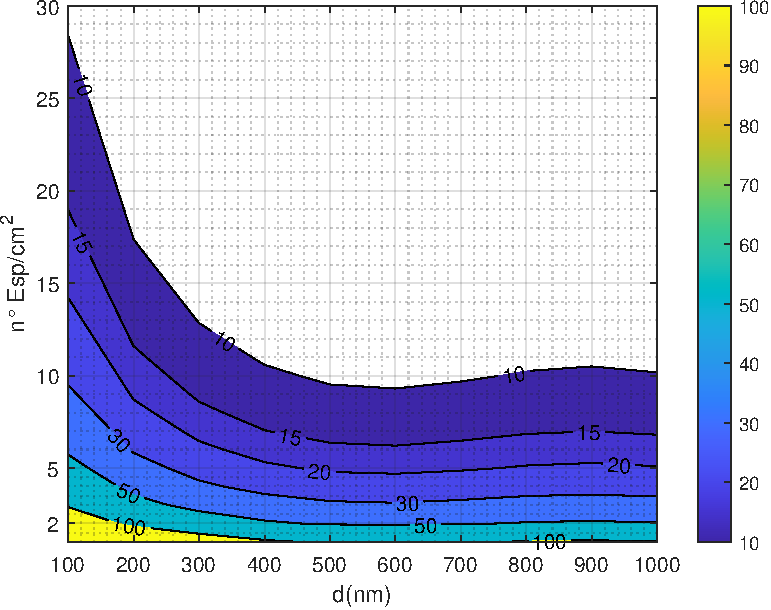
\includegraphics[width=\columnwidth]{rel_SiC}%
			\caption{}%
			\label{fig:prc_SiCSi}%
	\end{subfigure}
	\hfill
	\begin{subfigure}[b]{0.48\textwidth}%
			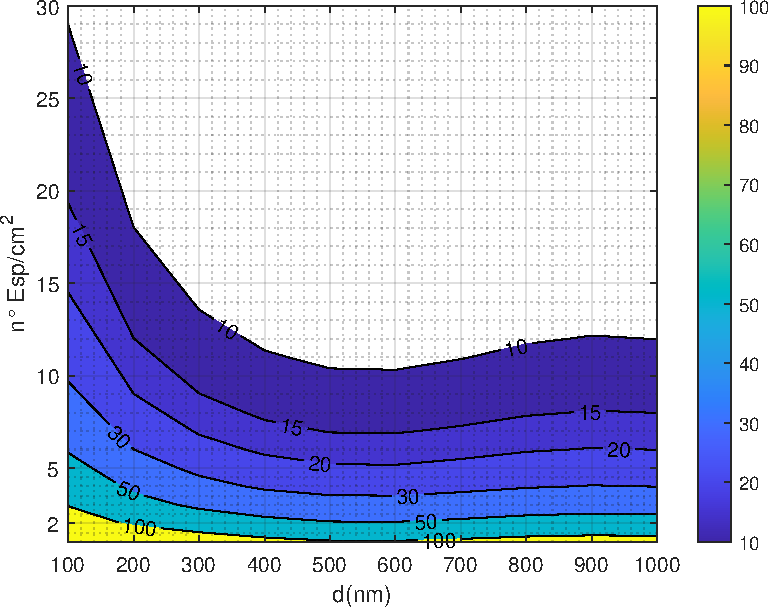
\includegraphics[width=\columnwidth]{SiC_Rc}%
			\caption{}%
			\label{fig:prc_SiCSiO2}%
	\end{subfigure}
	\caption{Densidades de nano-espaciadores ($n^{\circ}esp/cm^2$) frente a las alturas de los nano-espaciadores para todas las relaciones de la potencia de radiación en el rango espectral de energías mayores e igual a 0.7 eV respecto a las potencias de conducción con $R_c$ (dependientes en la densidad de nano-espaciadores) mayores a 10 para nTPVs de nano-espaciadores de $Si$ (\subref{fig:prc_SiCSi}) y $SiO_2$(\subref{fig:prc_SiCSiO2}) . Donde las barras de colores laterales de cada gráfica representan los colores asociados a cada uno de los valores de las relaciones de las potencias, con los contornos de las relaciones más significativas representadas en las gráficas.}%
	\label{fig:prc_SiCXX}%
\end{figure}
Por último, se calculan las densidades de nano-espaciadores frente a las alturas de los nano-espaciadores para la nTPV de emisor de $SiC$ y nano-espaciadores de $Si$, y se compara con las densidades de la nTPV de emisor de $SiC$ pero nano-espaciadores de $SiO_2$ (figuras \ref{fig:prc_SiCXX} \subref{fig:prc_SiCSi} y \subref{fig:prc_SiCSiO2}). Se observa que existe una disminución de las densidades para cada relación de potencias y todas las alturas de los nano-espaciaodores, siendo la más notable a los 1000nm de altura y relación de potencias de un orden de magnitud pasando la densidad de ser $12 \ n^{\circ}esp/cm^2$ (figura \ref{fig:prc_SiCSiO2}) a ser $10 \ n^{\circ}esp/cm^2$ (figura \ref{fig:prc_SiCSi}).